\documentclass{book}
\usepackage{fullpage}
\usepackage{amsfonts}
\usepackage{amssymb}
\usepackage{amsmath}
\usepackage{hyperref}
\usepackage{graphicx}% Include figure files
\usepackage{epstopdf}
\usepackage{subfig}
\usepackage{appendix}
%\usepackage{setspace}\doublespace
\author{Guojun Zhu}
\title{My Daily Note}
\newcommand{\vk}{\ensuremath{\mathbf{k}}}
\newcommand{\vK}{\ensuremath{\mathbf{K}}}
\providecommand{\vr}{\ensuremath{\mathbf{r}}}
%\newcommand{\vec}[1]{\ensuremath{\mathbf{#1}}}

\newcommand{\gk}{\ensuremath{{g}(\mathbf{k})}}

\newcommand{\vp}{\ensuremath{\mathbf{p}}}
\newcommand{\gp}{\ensuremath{{g}(\mathbf{p})}}

\newcommand{\vq}{\ensuremath{\mathbf{q}}}

\newcommand{\Fo}{\ensuremath{\mathbf{F_0}}}


\newcommand{\E}{\ensuremath{\mathbf{E}}}
\newcommand{\A}{\ensuremath{\mathbf{A}}}
\newcommand{\J}{\ensuremath{\mathcal{J}}}

\newcommand{\ket}[1]{\ensuremath{\left|#1\right>}}
\newcommand{\bra}[1]{\ensuremath{\left<#1\right|}}

\newcommand{\twoe}{\ensuremath{2\epsilon_\vk-\E_1}}

\newcommand{\nth}[1]{\ensuremath{\frac{1}{#1}}}

\newcommand{\br}[1]{\ensuremath{\left(#1\right)}}
\newcommand{\mbr}[1]{\ensuremath{\left[#1\right]}}
\newcommand{\bbr}[1]{\ensuremath{\left\{#1\right\}}}


\newcommand{\tk}{\ensuremath{\tilde{k}}}

\newcommand{\kp}{\ensuremath{\ket{\Psi}}}

\newcommand{\av}[1]{\ensuremath{\bigl<{#1}\bigr>}}
\newcommand{\avs}[3] {\av{#1{\lvert{#2}\rvert}#3}}
\newcommand{\avv}[2][\nu] {\avs{#1}{#2}{#1}}
\newcommand{\avt}[2]{\av{{#1}|{#2}}}
\newcommand{\avtu}[1]{\av{T_\tau#1}}

\newcommand{\Bop}{\ensuremath{\mathbf{B_0^+}}}
\newcommand{\Bmp}{\ensuremath{\mathbf{B_m^+}}}
\newcommand{\Bnp}{\ensuremath{\mathbf{B_n^+}}}
\newcommand{\Bo}{\ensuremath{\mathbf{B_0}}}
\newcommand{\Bopn}{\ensuremath{\mathbf{{B_0^+}^n}}}
\newcommand{\Bon}{\ensuremath{\mathbf{{B_0}^n}}}


\newcommand{\zmatrix}{\ensuremath{\br{\begin{smallmatrix}0&0\\0&0\end{smallmatrix}}}}
\newcommand{\fmtrx}[4]{\ensuremath{\br{\begin{smallmatrix}#1&#2\\#3&#4\end{smallmatrix}}}}
\newcommand{\smtrx}[6]{\ensuremath{\br{\begin{smallmatrix}#1&#2\\#3&#4\\#5&#6\end{smallmatrix}}}}

\newcommand{\vz}{\ensuremath{v^{\beta\alpha}_{\vk,\vk}}}


\providecommand{\abs}[1]{\ensuremath{\lvert{#1}\rvert}}

\newcommand{\sg}[1][1]{\ensuremath{\sigma_\frac{#1}{2}}}

\newcommand{\rhof}{\ensuremath{\rho(\ef)}}
\newcommand{\omt}{\ensuremath{\tilde{\Omega}}}
\newcommand{\cht}{\ensuremath{\tilde{\chi_0}}}
\newcommand{\Atl}{\ensuremath{\abs{A}^{2l}}}
\newcommand{\ef}{\ensuremath{\epsilon_F}}

\newcommand{\lca}{\ensuremath{\ln\br{1+\frac{\cht}{\alpha}}}}

\newcommand{\com}[2]{\ensuremath{\mbr{#1,#2}}}
\newcommand{\D}{\ensuremath{\mathit{D}}}
\newcommand{\dg}{\ensuremath{\dagger}}
\newcommand{\nG}{\ensuremath{\hat{\mathcal{G}}^{-1}}}

\providecommand{\lvk}{\ensuremath{1/\vk_F}}
\providecommand{\hm}{\ensuremath{\frac{\hbar^2}}{2m}}
\providecommand{\pdiff}[2]{\ensuremath{\frac{\partial{#1}}{\partial{#2}}}}
\providecommand{\dpdiff}[2]{\ensuremath{\frac{\partial^2{#1}}{\partial{{#2}^2}}}}

\providecommand{\H}{\ensuremath{\mathcal{H}}}
\providecommand{\wt}[1]{\widetilde{#1}}

\providecommand{\eef}[1]{Eq. (\ref{#1})}

\providecommand{\sch}{{Schr\"{o}dinger }}

\providecommand{\sgn}{\ensuremath{\text{sgn}}}
\newcommand{\Arctg}{\ensuremath{\text{Arctg}}}

\providecommand{\comm}[1]{\textit{\scriptsize \uwave{(#1)}}}
\renewcommand{\emph}[1]{\textbf{#1}}
\begin{document}
%\maketitle

%\tableofcontents
\numberwithin{equation}{section}


%\section{}
%\subsection{Two-Body Density Matrix in Richardson Solution}
As pointed in \cite{Leggett}, the existing of eigenvalue in order of $N$ in the two-body density matrix of BCS solution is probably the most fundamental fact of the superfluid phenomenon.  In the traditional BCS ansatz, the order parameter $F_\vk=u_\vk v^*_\vk$ is this eigenvector with the eigenvalue of $N_0=\frac{\pi}4\Delta{}N(0)\Omega$, \cite[(5.4.32)]{Leggett}.  Therefore it is important to check the solution with Richardson approach \cite{CobosonBcsRich} about this quantity.  What we are looking for is only zero-central-momentum eigenfunction, 
\begin{equation}\label{eq:2bodyDensityMatrixDef}
\av{\beta_\vk^\dg\beta_{\vk'}^{}}=\av{a_\vk^\dg{}b_{-\vk}^\dg{}b_{-\vk'}^{}{}a_{\vk'}^{}}
\end{equation}
Here we mostly follow the original paper's notion, with some short-hand explained as following:
\begin{equation}
 B^\dg_i=B^\dg(R_i)
\end{equation}
\begin{equation}
 \avt{i}{\vk}=\avv{B_i^{}\beta^\dg_\vk}
\end{equation}
\begin{equation}
 \avt{i}{j}=\avv{B_i^{}B^\dg_j}=\sum_\vk \avt{i}{\vk} \avt{\vk}{j}
\end{equation}

In the Richardson solution, ground wave-function is $\ket{\Psi_n}=\prod_i^n{}B^\dg_i\ket{\nu}$. Here different $B^\dg_i\ket{\nu}$'s are neither orthogonal nor normalized. In fact, they have rather substantial overlap most of the time.   Two-body density matrix here is further complicated by the fact that many-body wave-function is affected by the \emph{composite} nature of those cobosons. Generally,  
\begin{equation}
\av{\beta_\vk^\dg\beta_{\vk'}^{}}=\frac{\avv[\Psi_n]{\beta_\vk^\dg\beta_{\vk'}^{}}}{\avt{\Psi_n}{\Psi_n}}
\end{equation}.   

\subsubsection{Two pairs}
We started with a two-pair state, $\ket{\Psi_2}=B^\dg_i{}B^\dg_j\ket{\nu}$. 

\begin{equation}\label{eq:tbdm2pair}
\begin{split}
 &\avv[\Psi_2]{\beta_\vk^\dg\beta_{\vk'}^{}}\\
=&\mbr{\br{\avt{i}{j}\avt{j}{\vk}\avt{\vk'}{j}+\avt{i}{j}\avt{j}{\vk}\avt{\vk'}{i}}+(i\leftrightarrow{}j)}\\
  &-2\mbr{\br{\avt{j}{\vk}\avt{i}{\vk}\avt{\vk}{i}\avt{\vk'}{j}+\avt{\vk'}{i}\avt{\vk'}{j}\avt{j}{\vk}\avt{i}{\vk'}}+(i\leftrightarrow{}j)}\\
&+4\avt{j}{\vk}\avt{i}{\vk}\avt{\vk'}{i}\avt{\vk'}{j}\delta_{\vk\vk'}
\end{split}
\end{equation}
Here the first four terms (fig. \ref{fig:tbdm2pair1},\ref{fig:tbdm2pair2}) are from the paring, while the next eight terms (fig. \ref{fig:tbdm2pair3}-\ref{fig:tbdm2pair6}) as well as the last term  (fig. \ref{fig:tbdm2pair7}) are due to the Pauli exclusion of \emph{composite} nature. They show the moth-eaten effect.
\begin{figure}[htb]
\centering
  \subfloat[][]{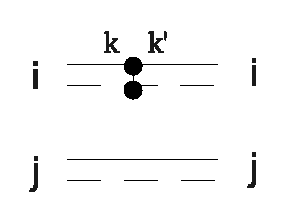
\includegraphics[width=0.2\textwidth]{image/tbdm2pair1.eps}\label{fig:tbdm2pair1}}\qquad
 \subfloat[][]{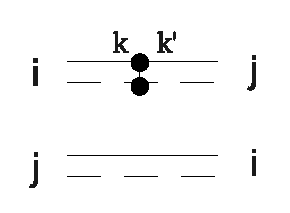
\includegraphics[width=0.2\textwidth]{image/tbdm2pair2.eps}\label{fig:tbdm2pair2}}\qquad
  \subfloat[][]{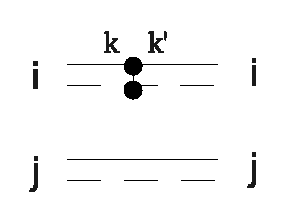
\includegraphics[width=0.2\textwidth]{image/tbdm2pair1.eps}\label{fig:tbdm2pair3}}\\
 \subfloat[][]{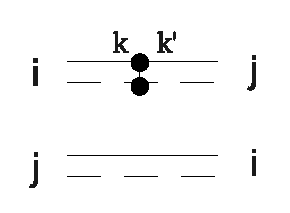
\includegraphics[width=0.2\textwidth]{image/tbdm2pair2.eps}\label{fig:tbdm2pair4}}\qquad
  \subfloat[][]{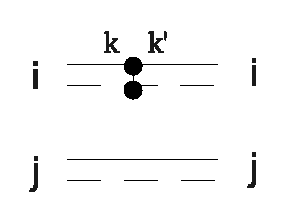
\includegraphics[width=0.2\textwidth]{image/tbdm2pair1.eps}\label{fig:tbdm2pair5}}\qquad
 \subfloat[][]{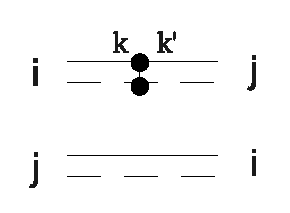
\includegraphics[width=0.2\textwidth]{image/tbdm2pair2.eps}\label{fig:tbdm2pair6}}\\
  \subfloat[][]{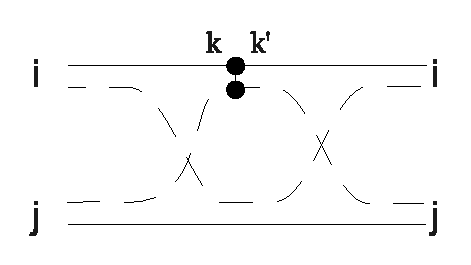
\includegraphics[width=0.3\textwidth]{image/tbdm2pair7.eps}\label{fig:tbdm2pair7}} 
\caption{Shiva diagram of two pairs }
\begin{description}
\item[\subref{fig:tbdm2pair1},\subref{fig:tbdm2pair2}] Signle pair without Pauli scattering.  There are also terms with $(i\leftrightarrow{j})$. First line of the above equation. 
\item[\subref{fig:tbdm2pair3},\subref{fig:tbdm2pair4},\subref{fig:tbdm2pair5},\subref{fig:tbdm2pair6}] Two-pair with Pauli scattering.  There are also terms with $(i\leftrightarrow{j})$. 
Second line of the equation. 
\item[\subref{fig:tbdm2pair7}] This coresponds the last term.  And there are the permutation of (i,j) as other terms.  
\end{description}
\end{figure}

The last term is especially interseting as this is two separate pieceses (fig.\ref{fig:shivaseparate}).  Normally, they do not exist, but here they do show up because we need pair of $\vk$,$\vk'$ .  
\begin{figure}[htb]\centering
 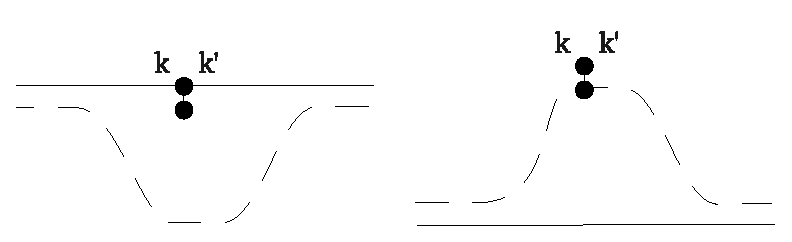
\includegraphics[width=0.3\textwidth]{image/shivaSeparate.eps}
\caption{Two separate connection parts of the last term of \eqref{eq:tbdm2pair}\label{fig:shivaseparate}}\centering
\end{figure}
And the normalization factor:
\begin{equation}
 {\avt{\Psi_2}{\Psi_2}}=\av{B^{}_j{}B^{}_i{}B^\dg_i{}B^\dg_j}=\avt{i}{i}\avt{j}{j}+\abs{\avt{i}{j}}^2-2\sum_\vk\avt{j}{\vk}\avt{i}{\vk}\avt{\vk}{i}\avt{\vk}{j}
\end{equation}

\subsubsection{Three pairs}
For a three-pair state $\ket{\Psi_3}=B^\dg_i{}B^\dg_j{}B^\dg_m\ket{\nu}$. 
we have 
\begin{equation}
\begin{split}
 \bra{\Psi_3}\beta^\dg_\vk=&\bra{\nu}B_m{}B_j{}B_i\beta^\dg_\vk\\
=&-2\avt{j}{\vk}\avt{m}{\vk}\bra{\nu}\beta_\vk{}B_i-2\avt{m}{\vk}\avt{i}{\vk}\bra{\nu}\beta_\vk{}B_j
-2\avt{i}{\vk}\avt{j}{\vk}\bra{\nu}\beta_\vk{}B_m\\
&+\avt{m}{\vk}\bra{\nu}B_i{}B_j+\avt{i}{\vk}\bra{\nu}B_j{}B_m+\avt{i}{\vk}\bra{\nu}B_m{}B_i\\
=&\br{-2\avt{i}{\vk}\avt{j}{\vk}\bra{\nu}\beta_\vk{}B_m+\avt{i}{\vk}\bra{\nu}B_j{}B_m}+(\mbox{i,j,m rotate permutation})
\end{split}
\end{equation}
We are lots of terms in the final expectation, like $\av{B^\dg{}B^\dg{}B^{}B^{}}$, $\av{\beta^\dg{}B^\dg{}B^{}B^{}}$,$\av{\beta^\dg{}B^\dg{}B^{}\beta^{}}$ , $\av{B^\dg{}B^\dg{}B^{}\beta^{}}$ .  
%\subsection{Variation method with the u,v,w}
We start with three hyperfine species a, b, c, where a is the common species in two channel. (a,b) is the open channel while (a,c) is the close channel. And the Hamiltonian is written in the form 
\begin{equation}
\begin{split}
 H=&\sum_\vk\epsilon^a_\vk{}a^+_\vk{}a^{}_\vk+\sum_\vk\epsilon^b_\vk{}b^+_\vk{}b^{}_\vk+\sum_\vk\epsilon^c_\vk{}c^+_\vk{}c^{}_\vk\\
  &+\nth{2}\sum_{\vk\vk'}U_{\vk\vk'}a^+_\vk{}b^+_{-\vk}{}b^{}_{-\vk'}a^{}_{\vk'}
	+\nth{2}\sum_{\vk\vk'}V_{\vk\vk'}a^+_\vk{}c^+_{-\vk}{}c^{}_{-\vk'}a^{}_{\vk'}\\
 &+\nth{2}\sum_{\vk\vk'}Y_{\vk\vk'}a^+_\vk{}b^+_{-\vk}{}c^{}_{-\vk'}a^{}_{\vk'}
	+\nth{2}\sum_{\vk\vk'}Y^*_{\vk\vk'}a^+_{\vk'}{}c^+_{-\vk'}{}b^{}_{-\vk}a^{}_{\vk}
\end{split} 
\end{equation}
By the Hermition condition we have 
\begin{equation}
 U_{\vk'\vk}=U^*_{\vk\vk'},\qquad{} V_{\vk'\vk}=V^*_{\vk\vk'}
\end{equation}
  We start from the ansatz as 
\begin{equation}\label{eq:ansatz}
 \ket{\Psi}=\prod_\vk\br{u_\vk+v_\vk{}a^\dg_\vk{}b^\dg_{-\vk}+w_\vk{}a^\dg_\vk{}c^\dg_{-\vk}}\ket{0}
\end{equation}
Here we require $\abs{u_\vk}^2+\abs{v_\vk}^2+\abs{w_\vk}^2=1$ for normalization.  For all the interaction term, there are two types of contribution,
for example, 
\begin{equation*}
\av{U_{\vk\vk'}a^\dg_\vk{}b^\dg_{-\vk}{}b^{}_{-\vk'}a^{}_{\vk'}}
=\sum_{\vk}U_{\vk\vk}\abs{v_\vk}^2+\sum_{\vk\neq\vk'}U_{\vk\vk'}v^{}_{\vk'}u^*_{\vk'}u^{}_\vk{}v^*_\vk
\end{equation*}
The first term is the Hatree term and the second term is more interesting pairing term.



And the free energy is 
\begin{equation}
 \begin{split}
  &F\equiv\av{H-\mu{}N}\\
    =&\sum(\xi^a_\vk+\xi^b_\vk)\abs{v_\vk}^2+\sum(\xi^a_\vk+\xi^c_\vk)\abs{w_\vk}^2\\
    &+\nth2\sum_{\vk}U_{\vk\vk}\abs{v_\vk}^2+\nth2\sum_{\vk\neq\vk'}U_{\vk\vk'}v^{}_{\vk'}u^*_{\vk'}u^{}_\vk{}v^*_\vk\\
    &+\nth2\sum_{\vk}V_{\vk\vk}\abs{w_\vk}^2
      +\nth2\sum_{\vk\neq\vk'}V_{\vk\vk'}w^{}_{\vk'}u^*_{\vk'}u^{}_\vk{}w^*_\vk\\
    &+\nth2\sum_{\vk}Y_{\vk\vk}w^{}_{\vk}v^*_\vk{}
      +\nth2\sum_{\vk\neq\vk'}Y_{\vk\vk'}w^{}_{\vk'}{u^{*}_{\vk'}}v^*_\vk{}u^{}_\vk\\
    &+\nth2\sum_{\vk}Y^*_{\vk\vk}w^*_{\vk}v^{}_{\vk}{}
      +\nth2\sum_{\vk\neq\vk'}Y^*_{\vk\vk'}w^*_{\vk}{u^{}_{\vk}}v^{}_{\vk'}{}u^{*}_{\vk'}
 \end{split}
\end{equation}
Where 
\begin{equation*}
 \xi^a_\vk=\epsilon^a_\vk-\mu^a,\qquad\xi^b_\vk=\epsilon^b_\vk-\mu^b,\qquad\xi^c_\vk=\epsilon^c_\vk-\mu^b
\end{equation*}
The chemical potential is added to make sure the $n_a=n_b+n_c=\nth{2}n$.
 I drop the Hatree term as this in some sense just shift the chemical potentials as it only relates to the density.  (\emph{Not sure still valid in the two-channel problems, especially for the close-channel.})  Also, I ignore the summation on the second only goes through $\vk\neq\vk'$ as the correction is in the higher order. 
 
Now introduce the parameters $\theta_\vk$, $\phi_\vk$ to include the normalization condition.  
\begin{equation}
 u_{\vk}=\cos\theta_\vk,\qquad{} v_{\vk}=\sin\theta_\vk\cos\phi_\vk,\qquad{}
 w_{\vk}=\sin\theta_\vk\sin\phi_\vk
\end{equation}
We take them as real quantities as those that minimize the free energy are real.(?) Now the free energy can be written as 

\begin{equation}
 \begin{split}
  F=&\sum\xi^{ab}_\vk\sin^2{\theta_\vk}\cos^2\phi_\vk+\sum\xi^{ac}_\vk\sin^2{\theta_\vk}\sin^2\phi_vk\\
    &+\nth2\sum_{\vk\vk'}U_{\vk\vk'}\cos\theta_{\vk'}\sin\theta_{\vk'}\cos\phi_{\vk'}\cos\theta_\vk{}\sin\theta_\vk\cos\phi_\vk\\
    &+\nth2\sum_{\vk\vk'}V_{\vk\vk'}\cos\theta_{\vk'}\sin\theta_{\vk'}\sin\phi_{\vk'}\cos\theta_\vk{}\sin\theta_\vk\sin\phi_\vk\\
    &+\nth2\sum_{\vk\vk'}Y_{\vk\vk'}\cos\theta_{\vk'}\sin\theta_{\vk'}\cos\phi_{\vk'}\cos\theta_\vk{}\sin\theta_\vk\sin\phi_\vk\\
    &+\nth2\sum_{\vk\vk'}Y^*_{\vk\vk'}\cos\theta_{\vk'}\sin\theta_{\vk'}\sin\phi_{\vk'}\cos\theta_\vk{}\sin\theta_\vk\cos\phi_\vk\\
    =&\nth4\sum_\vk\xi^{ab}_\vk(1-\cos2\theta_\vk)(1+\cos2\phi_\vk)+\nth4\sum_\vk\xi^{ac}_\vk(1-\cos2\theta_\vk)(1-\cos2\phi_\vk)\\
    &+\nth{8}\sum_{\vk\vk'}U\sin2\theta_\vk\cos\phi_\vk\sin2\theta_{\vk'}\cos\phi_{\vk'}+\nth{8}\sum_{\vk\vk'}V\sin2\theta_\vk\sin\phi_\vk\sin2\theta_{\vk'}\sin\phi_{\vk'}    \\
    &+\nth{4}\sum_{\vk\vk'}Y\sin2\theta_\vk\cos\phi_\vk\sin2\theta_{\vk'}\sin\phi_{\vk'}    
 \end{split}
\end{equation}
We assume that $Y=Y^*$. From the above equation, we can differentiate it with respect to $\theta_\vk$ and $\phi_\vk$ and set the derivative as 0, therefore minimize free energy. 
\begin{align}
0=&\pdiff{F}{\theta_\vk}\notag\\
 =&\nth{2}\sin2\theta_\vk\mbr{\xi^{ab}_\vk(1+\cos2\phi_\vk)+\xi^{ac}_\vk(1-\cos2\phi_\vk)}\notag\\
 &+\nth2\sum_{\vk'}\cos2\theta_\vk\sin2\theta_{\vk'}\mbr{U\cos\phi_\vk\cos\phi_{\vk'}+V\sin\phi_\vk\sin\phi_{\vk'}+Y\sin(\phi_{\vk'}+\phi_\vk)}\\
 0=&\pdiff{F}{\phi_\vk}\notag\\
 =&-\nth{2}(\xi^{ab}_\vk-\xi^{ac}_\vk)\sin2\phi_\vk(1-\cos2\theta_\vk)\notag\\
 &-\nth4\sum_{\vk'}\sin2\theta_\vk\sin2\theta_{\vk'}\mbr{U\sin\phi_\vk\cos\phi_{\vk'}-V\cos\phi_\vk\sin\phi_{\vk'}-Y\cos(\phi_{\vk'}+\phi_\vk)}
\end{align}
  These two set of equations (for each $\vk$, but decoupled) fully determine the wave-function. 
We introduce two quantities:
\begin{align}
\Delta_\vk^U&=\sum_{\vk'}\sin2\theta_{\vk'}(U_{\vk\vk'}\cos\phi_{\vk'}+Y_{\vk\vk'}\sin\phi_{\vk'})\label{eq:gap1}\\
\Delta_\vk^V&=\sum_{\vk'}\sin2\theta_{\vk'}(V_{\vk\vk'}\sin\phi_{\vk'}+Y_{\vk\vk'}\cos\phi_{\vk'})\label{eq:gap2}
\end{align} 
As we can see eqs.(\ref{eq:gap1},\ref{eq:gap2}) is indeed very similar to the structure of two-body Schr\"{o}‌dinger equation.
If we ‌introduce the Zeeman energy detuning between two channels
\begin{equation}
\eta=\xi^{ab}-\xi^{ac}
\end{equation}
These equations can be written into a more compact form
\begin{align}
\tan2\theta_\vk&=-\frac{\cos\phi_\vk\Delta^U_\vk+\sin\phi_\vk\Delta^V_\vk}{2\xi^{ab}_\vk+2\eta\cos^2\phi_\vk}\label{eq:tan1}\\
\tan\theta_\vk&=-\frac{\sin\phi_\vk\Delta^U_\vk-\cos\phi_\vk\Delta^V_\vk}{2\eta\sin2\phi_\vk}\label{eq:tan2}
\end{align} 


Furthermore, when $k\rightarrow\infty$, from eq. (\ref{eq:tan1}), we see that $\theta\rightarrow0$ as $1/\xi$;  and from eq. (\ref{eq:tan2}), we see that $\sin\phi_\vk\Delta^U=\cos\phi_\vk\Delta^V$ as we assume $\Delta$ varies slowly over $\vk$.  We have 
\begin{align*}
\cos^2\phi_\vk&=\frac{{\Delta^U}^2}{{\Delta^V}^2+{\Delta^U}^2}\\
\sin^2\phi_\vk&=\frac{{\Delta^V}^2}{{\Delta^V}^2+{\Delta^U}^2}
\end{align*}
And 
\[\tan2\theta_\vk=-\frac{({{\Delta^V}^2+{\Delta^U}^2})^{1/2}}{2\xi^{ab}_\vk}\]

Eqs. (\ref{eq:gap1},\ref{eq:gap2}) are similar as those derived from the Green's function method in the eq. (\ref{eq:gapMatrix}), and should be able to renormalized in the similar fashion $\Delta=T(F-G\Delta)$, where in our notation $({F^o,F^c})=(\cos\theta_\vk\sin\theta_\vk\cos\phi_\vk,\cos\theta_\vk\sin\theta_\vk\sin\phi_\vk)$.  The problem, however, is that the eqs. (\ref{eq:tan1},\ref{eq:tan2}) does not present a simple analytic solution about $\theta$ and $\phi$ in terms of $\Delta$ and therefore the gap equations cannot be written into a simple renormalized  equation although they are implicit functions of $\Delta$.
 It is a rather cumbersome process to calculate the integration in renormalized gap equations.  Furthermore, information of the close-channel is close to a simple one-level bound-state is not fully incorporated and the equation might be simpler and has a nicer form if I can manage to do that.  

\subsection{more thoughts}
From eqs. (\ref{eq:gap1},\ref{eq:gap2}), $\Delta^{U,V}_\vk$ varies slowly with $k$ if interaction depends on momentum weakly, at least for low momentum.  Therefore, in the renomalization, they can be taken as constants.  In that case, eqs. (\ref{eq:tan1},\ref{eq:tan2}) determine $\theta_k(\xi_k,\Delta^U,\Delta^V)$ and $\phi_k(\xi_k,\Delta^U,\Delta^V)$, which in turn give two-body wave-function $F^{o,c}_k(\xi_k,\Delta^U,\Delta^V)$.  
With the renomalized gap equation,.  
\begin{equation}\label{eq:renomal1}
\begin{pmatrix}\Delta^U\\\Delta^V\end{pmatrix}=\begin{pmatrix}T_{oo}&T_{oc}\\T_{co}&T_{cc}\end{pmatrix}
\begin{pmatrix}\sum{F^o-\frac{\Delta^U}{2\epsilon}}\\\sum{F^c-\frac{\Delta^V}{2\epsilon+\eta}}\end{pmatrix}
\end{equation}
and the number equation, should give us three parameters in the problems: $\Delta^{U,V}$ and $\mu$.  The close-channel infomation is incorporated into the $T$-matrix.  The problem is more about the computation difficulty as there is no simple analytic solution for $F^{o,c}$, therefore, eq. (\ref{eq:renomal1}) cannot be done easily.

What happened in the broad-resonance limit? Or very BEC/BCS end? 

\subsection{T-matrix}
Follow \cite{JacksonNarrow}, the bare interaction $V$ should have the form \footnote{notice the some change of notation}
\begin{equation}
V(r)=\frac{V_s(r)+3V_t(r)}{4}+\mbr{V_t(r)-V_s(r)}\mathbf{S_1}\cdot\mathbf{S_2}
\end{equation}
we can establish the T-matrix from $V$.
\begin{equation}
 {\fmtrx{T_{cc}}{T_{co}}{T_{oc}}{T_{oo}}}^{-1}={\fmtrx{V_{cc}}{V_{co}}{V_{oc}}{V_{oo}}}^{-1}-{\fmtrx{G_{c}}{0}{0}{G_{o}}}
\end{equation}
For 0-temperature, pair propagators $G_o$ and $G_c$ are
\begin{equation}
 G_o(\omega,\vK,\vq)=\nth{\omega+i\delta-\frac{K^2}{4m}-\frac{q^2}{m}}
\end{equation}
\begin{equation}
 G_c(\omega,\vK,\vq,B)=\nth{\omega+i\delta-\eta(B)-\frac{K^2}{4m}-\frac{q^2}{m}}
\end{equation}
where $E_{th}(B)$ is the detuning, depending on magnatic field $B$. Here we can break it down into two steps. First, introduce 
 \begin{equation}
 {\fmtrx{U_{cc}}{U_{co}}{U_{oc}}{U_{oo}}}^{-1}={\fmtrx{V_{cc}}{V_{co}}{V_{oc}}{V_{oo}}}^{-1}-{\fmtrx{G^{vac}}{0}{0}{G^{vac}}}
\end{equation}
where $G^{vac}(q)=(i\delta-q^2/m)^{-1}$ is the vacuum pair propagator ignoring the hyperfine splitting at $\omega=0$ and no center momentum $\vK$.  Furthermore, when the close-channel resonnant state is close to threshold and well-seperated from other discrete levels, the effective interaction is separable.  So 
\begin{equation}
 U(\vq',\vq)=\frac{4\pi}{m}\mbr{\frac{a_s+3a_t}{4}+(a_t-a_s)\mathbf{S_1}\cdot\mathbf{S_2}}g(q')g(q)
\end{equation}
$g(q)\rightarrow0$ for $qr_C\rightarrow\infty$ where $r_C$ is the interaction range.  But This can be projected to the hyperfine-spin space and therefore two-channel.  
\begin{equation}
 {\fmtrx{U_{cc}}{U_{co}}{U_{oc}}{U_{oo}}}=
\frac{4\pi}{m}\mbr{\fmtrx{\frac{c_7a_s+a_t}{1+c_7}}{\frac{a_t-a_s}{\sqrt{1+c_7}\sqrt{1+c_9}}}
{\frac{a_t-a_s}{\sqrt{1+c_7}\sqrt{1+c_9}}}{\frac{c_9a_s+a_t}{1+c_9}}}
\end{equation}
For example, $\ket{9/2,-9/2}$, $\ket{9/2,-7/2}$, $\ket{7/2,-7/2}$ of ${}^{40}K$ at resonance $B=201.6$, $c_7=14.9$ and $c_9=0.059$ Note that both $c_7$ and $c_9$ depends on B.  

The second step deals with the influence of $B$ in the theshold $E_{th}$ as well as the energy dependence of $G$. 
 \begin{equation}
  {\fmtrx{T_{cc}}{T_{co}}{T_{oc}}{T_{oo}}}^{-1}={\fmtrx{U_{cc}}{U_{co}}{U_{oc}}{U_{oo}}}^{-1}-{\fmtrx{\Delta{}G_c}{0}{0}{\Delta{}G_o}}
\end{equation}
where $\Delta{}G_{o/c}=G_{o,c}(\omega,\vK,\vq,B)-G^{vac}(q)$.  Using the seperable properties of $U$, we can concentrate the $\vq$ dependence on two quantities and this leaves us a simple two-by-two algebra matrix equation.  
\begin{equation}
\Pi_{o,c}(\omega,\vK,B)=\int\frac{d^3q}{(2\pi)^3}\Delta{}G_{o,c}g^2(q)                  
\end{equation}
where for the contact interaction with $r_C=0$, we find $\Pi_o(\omega,\vK)=-im^{3/2}\sqrt{\omega-K^2/(4m)}$ and $\Pi_c(\omega,\vK,B)=\Pi_o(\omega-E_{th}(B),\vK)$
Especially, for $\omega=0$ and no central mometum $\vK$, $\Pi_o=0$ and $\Pi_c=\sqrt{-\eta(B)}$
\begin{gather}\label{eq:T}
 T_{cc}=\frac{U_{cc}}{1-U_{cc}\Pi_c}\\
T_{oc}=T_{co}=\frac{U_{oc}}{1-U_{cc}\Pi_c}\\
T_{oo}=U_{oo}+\frac{U_{oc}^2\Pi_c}{1-U_{cc}\Pi_c}
\end{gather}
comparing this with the commonly used formula 
\begin{equation}
 T_{oo}=\frac{4\pi{}a_{bg}}{m}\br{1-\frac{\Delta{}B}{B-B_0}}
\end{equation}
We find the resonance position $B_0$ satisfies
\begin{equation}
 1-U_{cc}(B_0)\Pi_c(B_0)=0
\end{equation}
And other quantities, such as $a_s$, $a_t$ can be expressed with the experimental quantities. 

However, it is still not clear to me how to really map broad /narrow resonance into the many-body eq.(\ref{eq:renomal1}) in a calculable sense.  The criteria of broad resonance as in \cite{JacksonNarrow} is   
\begin{equation}\label{eq:broadCriteria}
\Delta\mu\Delta{}B\gg\frac{k_F}{ma_{bg}}
\end{equation}


\subsection{rescale with Fermi momemtum/energy}
If we rescale renormalized gap equation eq. \ref{eq:renomal1} and the number equation with the Fermi momentum/energy, we have 
\begin{equation}\label{eq:renormal2}
\begin{pmatrix}\widetilde\Delta^U\\\widetilde\Delta^V\end{pmatrix}=
8\pi{a}{k_F}\begin{pmatrix}1&T_{oc}/T_{oo}\\T_{co}/T_{oo}&T_{cc}/T_{oo}\end{pmatrix}
\int\widetilde{k}^2d\widetilde{k}
\begin{pmatrix}
\nth{2}\sin2\theta_{k}\cos\phi_k-\frac{\widetilde\Delta^U}{2\widetilde\epsilon}\\
\nth{2}\sin2\theta_{k}\sin\phi_k-\frac{\widetilde\Delta^U}{2\widetilde\epsilon+\widetilde{\eta}}
\end{pmatrix}
\end{equation}
and rescaled number equation
\begin{equation}
 \int\widetilde{k}^2\sin^2\theta_kd\widetilde{k}=\nth{3}
\end{equation}
We can find the criteria of broad resonance (eq. \ref{eq:broadCriteria}) becomes 
\begin{equation}
 ak_F\widetilde{\eta}\gg1 
\end{equation}
Here we use $a=a_{bg}(1+\Delta_B/(B-B_0)$,  ignoring constant $1$ around the resonance, and also use the fact that rougly $\eta=\Delta\mu(B-B_0)$. At the broad limit, term $\frac{\widetilde\Delta^U}{2\widetilde\epsilon+\widetilde{\eta}}$ of the second integration in eq. \ref{eq:renormal2} gives a negligible contribution when $\sin2\theta_k$ is substantial.  So a simple solution is to put $\cos\phi_k\approx1$ while $\sin\phi_k\approx0$ for where $\sin2\theta_k$ is substantial (i.e. the particle is concentrated in open-channel).  Therefore, we reduce the two-channel problems into one-channel problem, omitting the close-channel. Here, we can see the interplaying between fermi energy and the two-body quantities, whether eq. \ref{eq:renormal2} can be reduced to a single-channel problem is due to the size of $\widetilde{\eta}$, which is determined by the ratio of the deturning and Fermi energy.  
%\section{note of 2009.12.07}
%\subsection{Spherical harmonic and Fourier transformation}
From (34.3) of \cite{landau}, we have
\begin{equation}
e^{i\vk\cdot\vr}=4\pi\sum_{l=0}^{\infty}\sum_{m=-l}^{l}i^l{}j_l(kr)Y^*_{lm}(\hat{k})Y_{lm}(\hat{r})
\end{equation}
We find the the Fourier tansformation in 3D of the spherical harmonic function does not change $(lm)$,
\begin{equation}
\int{d\hat{k}e^{i\vk\cdot\vr}Y_{lm}(\hat{k})}=4\pi{}i^l{}j_l(kr)Y_{lm}(\hat{r})
\end{equation} 
And 
\begin{equation*}
\Psi(\vr)=\sum_{l=0}^{\infty}\sum_{m=-l}^{l}\int{dk}\psi_{lm}{(k)}\int{d\hat{k}e^{i\vk\cdot\vr}Y_{lm}(\hat{k})}=4\pi{}\sum_{l=0}^{\infty}\sum_{m=-l}^{l}i^l{}Y_{lm}(\hat{r})\int{dk}\psi_{lm}{(k)}j_l(kr)
\end{equation*}
So the $(lm)$ component of real-space relates only to the $(lm)$ component of k-space 
\begin{equation}
\psi_{lm}(r)=4\pi{}i^l{}\int{dk}\psi_{lm}{(k)}j_l(kr)
\end{equation}


\subsection{Shizhong's comment\label{subsec:20091207}}
He think besides open-channel affects close-channel in statistics, there is also the statistical effect from close-channel to open-channel.  And finally, one can include both coherently. Numerically, one can do these two things iterately and maybe find the many-body result. There are also kinetical interaction and the full treatment involve the $2\times2$.   

\textit{My thinking:The assumption that close-channel molecule is large and close-to-threshhold, actually increases the statistical effect of close-channel to open-channel because close-channel is then denser in k-space.  	}

He has doubts to characterize the close-channel bound-state with one single parameter $a_s$, but he agrees that this might be OK for a model.  I think it is fine given the condition that close-channel is close-to-threshold and very large.  

%\section{Scattering amplitude and scattering length for our model \label{sec:scatter}}
In dilute system or short-range potential, low-energy property of the potential can be described with scattering amplitude\cite{Pethick,Fetter}, more specifically, s-wave scattering length $a_{s}$ is routinely used to describe the potential in atomic physics, where most problems is only about very low energy and low density.  So it is interesting to find the scattering amplitude and s-wave scattering length for our model potential. We notice that our model is actually very similar as the one-channel model used by Gurarie and Radzihovsky (sec. 3 and sec. 4.1 of Ref. \cite{GurarieNarrow}). 

Scattering amplitude, or, T-matrix can be written as 
\begin{equation}
-\frac{4\pi}{mL^3}f_{\vk\vk'}=T_{\vk\vk'}=[\frac{U}{(1-U\Pi)}]_{\vk\vk'}
\end{equation}
where $\Pi$ is the propagator of a pair.  In a translation invariant system with central potential, all quantities depend $\vk$ and $\vk'$ only through $\vk-\vk'$ and we can separate the solution into different partial wave. Especially for the s-wave, the complicated  integral becomes a simple number,
\begin{equation}
T^{0}_{k}=\frac{u^{0}_{k}}{1-u^{(0)}_{k}\Pi^{(0)}(\epsilon_k)}
\end{equation}
Here 
\begin{equation}
\begin{split}
\Pi^{(0)}(\epsilon)=&\int\frac{d^{3}\vq}{{(2\pi)}^{3}}\frac{w_{k}}{\epsilon-q^{2}/m+i0}\\
=&-\frac{m}{2\pi^{2}}{\Lambda}+\frac{m\sqrt{\epsilon{m}}}{2\pi^{2}}\arctan\frac{\Lambda}{\sqrt{\epsilon{m}}}\\
&-i\frac{m^{3/2}}{4\pi}\sqrt{\epsilon}
\end{split}
\end{equation}
Where $\Lambda$ is the cutoff in momentum, $\Lambda^{2}/(2m)\equiv\Omega$. The second term is small compared to the first term when the cutoff is large, so we will ignore it.  In our model, $u^{0}_{k}=-vw_{k}$, And we find the scattering amplitude 
\begin{equation}
f_{s}(k)=-\frac{1}{-\frac{4\pi}{mv}+\frac{2\Lambda}{\pi}+ik}
\end{equation}
and s-wave scattering length is its limit at zero energy. 
\begin{equation}
\begin{split}
a(v)=&\left(-\frac{4\pi}{mv}+\frac{2\Lambda}{\pi}\right)^{-1}\equiv\frac{m}{4\pi}v_{R}\\
     =&\frac{m}{4\pi}\frac{-v}{1-v/v_{c}}
     \end{split}
\end{equation}
where $v_{R}$ can be called renormalized coupling and 
\begin{equation}
v_{c}=\frac{2\pi^{2}}{\Lambda{m}}
\end{equation}
We find that, for large attractive, i.e., for $v$ large and position, $a\approx\frac{m}{4\pi}v_c$ is small positive as $\Lambda$ is large and increases as attraction decrease, it diverges at $v=v_{c}$ and which is the same as our threshold $v^{\text{th}}(1)$.  When $v$ gets even smaller, there is no bound-state and $a$ becomes large negative and its absolute value decease as $v$ decrease until $a(v=0)=0$. 
$a(v)$ can also be written as
\begin{equation}
a(v)=\frac{\pi}{2\Lambda}\left(1-\frac{2\pi^{2}}{mv\Lambda}\right)^{-1}
\end{equation}
This can be easily related to binding energy by $E_{b}=-1/(ma^{2})$ when close to threshold. 
%\subsection{Note about scale of $a_{s}$, $f$ and $T$}
\begin{itemize}
\item $a_{s}=-\lim_{k\rightarrow0}f_{k}$, so $a_{s}$ scales as $f_{k}$;
\item In a collision problem, the scattering wave-function has asymptotic form
\begin{equation}\label{eq:relation:Psi}
\Psi^{\prime}\sim{}e^{{i\vk\cdot\vr}}+f_{\vk}(\Omega)\frac{e^{ikr}}{r}
\end{equation}
It is easy to see that $f_{\vk}$ has the dimension of length.
\item $T$-matrix has the same dimension as interaction $V$.  However, $T_{{\vk\vk'}}=\avs{\phi_\vk(\vr)}{T}{\phi_\vk'(\vr)}$, the matrix element has dimension of $\text{energy}\cdot\text{volume}$ if we use the normalization as Eq. \eqref{eq:relation:Psi}, which is quite common in scattering theory. And this is consistent with 
\begin{equation}
T_{\vk\vk'}=\frac{4\pi\hbar^{2}}{m}f_{\vk\vk'}
\end{equation}
 \item  All these quantities are two-body quantities.  (T can be used for many-body as well, but here we use it in two-body sense.) Their value should not depend on volume.  There seems to be some dependence because $\ket{\phi_{vk}(\vr)}$ only normalized in box-normalization, but the overall result should not depend on volume with a realistic potential.  
\end{itemize}

%\subsection{Fermionic Excitation in Three-Species Hamiltonian\label{sec:fermionicExcitation}}
Here we try to find the fermionic excitation for three-species system with reduced Hamiltonian via Bogoliubov canonical transformation\cite{Tinkham}
\begin{equation}\label{eq:threeReducedHamiltonian}
\begin{split}
 H=&\sum_\vk\epsilon^a_\vk{}a^+_\vk{}a^{}_\vk+\sum_\vk\epsilon^b_\vk{}b^+_\vk{}b^{}_\vk+\sum_\vk\epsilon^c_\vk{}c^+_\vk{}c^{}_\vk\\
  &+\nth{2}\sum_{\vk\vk'}U_{\vk\vk'}a^+_\vk{}b^+_{-\vk}{}b^{}_{-\vk'}a^{}_{\vk'}
	+\nth{2}\sum_{\vk\vk'}V_{\vk\vk'}a^+_\vk{}c^+_{-\vk}{}c^{}_{-\vk'}a^{}_{\vk'}\\
 &+\nth{2}\sum_{\vk\vk'}Y_{\vk\vk'}a^+_\vk{}b^+_{-\vk}{}c^{}_{-\vk'}a^{}_{\vk'}
	+\nth{2}\sum_{\vk\vk'}Y^*_{\vk\vk'}a^+_{\vk'}{}c^+_{-\vk'}{}b^{}_{-\vk}a^{}_{\vk}
\end{split} 
\end{equation}
Here $a$, $b$, $c$ are three species where $a$ is the common species between two channels. In principle, each specie has different magnetic moment and $\epsilon^{i}_{\vk}=\hbar^{2}k^{2}/2m+\mu^{i}B$. This hamiltonian is reduced in the sense that it has only zero-central-momentum component.  This is sufficient to find fermionic excitation though.(At least in the case of simple one-channel problem.)  We first linearize the hamiltonian with the mean-field value. For a superfluid system, we have non-zero mean-field value for anomalous quantities $F^{*}_{\vk}\equiv\av{a^+_\vk{}b^+_{-\vk}{}}$ and $G^{*}_{\vk}\equiv\av{a^+_\vk{}c^+_{-\vk}{}}$ and their complex conjugates. 
\begin{equation}
\begin{split}
 H=&\sum_\vk\epsilon^a_\vk{}a^+_\vk{}a^{}_\vk+\sum_\vk\epsilon^b_\vk{}b^+_\vk{}b^{}_\vk+\sum_\vk\epsilon^c_\vk{}c^+_\vk{}c^{}_\vk\\
  &+\nth{2}\sum_{\vk\vk'}U_{\vk\vk'}(F_{\vk'}a^+_\vk{}b^+_{-\vk}{}+F^{*}_{\vk}{}b^{}_{-\vk'}a^{}_{\vk'}+F_{\vk}^{*}F_{\vk'})\\
	&+\nth{2}\sum_{\vk\vk'}V_{\vk\vk'}(G_{\vk'}a^+_\vk{}c^+_{-\vk}{}+G^{*}_{\vk}c^{}_{-\vk'}a^{}_{\vk'}+G_{\vk}^{*}G_{\vk'})\\
 &+\nth{2}\sum_{\vk\vk'}Y_{\vk\vk'}(G_{\vk'}a^+_\vk{}b^+_{-\vk}{}+F^{*}_{\vk}c^{}_{-\vk'}a^{}_{\vk'}+F_{\vk}^{*}G_{\vk'})\\
	&+\nth{2}\sum_{\vk\vk'}Y^*_{\vk\vk'}(F_{\vk}a^+_{\vk'}{}c^+_{-\vk'}{}+G^{*}_{\vk'}b^{}_{-\vk}a^{}_{\vk}+G_{\vk}^{*}F_{\vk'})
\end{split} 
\end{equation}
This equation decoupled $\vk$ from all other momentum component.  $H=\sum_{\vk}h_{\vk}$, and each momentum compoennt $h_{\vk}$ can be simplified 
\begin{equation*}
\begin{split}
 h_{\vk}=&\quad\nth{2}\sum_{\vk'}(U_{\vk\vk'}F_{\vk}^{*}F_{\vk'}+V_{\vk\vk'}G_{\vk}^{*}G_{\vk'}
 +Y_{\vk\vk'}F_{\vk}^{*}G_{\vk'}+Y^*_{\vk\vk'}G_{\vk}^{*}F_{\vk'})\\
 &+\epsilon^a_\vk{}a^+_\vk{}a^{}_\vk+\epsilon^b_\vk{}b^+_\vk{}b^{}_\vk+\epsilon^c_\vk{}c^+_\vk{}c^{}_\vk\\
  &+\nth{2}\sum_{\vk'}(U_{\vk\vk'}F_{\vk'}+Y_{\vk\vk'}G_{\vk'})a^+_\vk{}b^+_{-\vk}{}+\nth{2}\sum_{\vk'}(U_{\vk'\vk}F^{*}_{\vk'}+Y^{*}_{\vk'\vk}G_{\vk'})b^{}_{-\vk}a^{}_{\vk}\\
ity  &+\nth{2}\sum_{\vk'}(V_{\vk\vk'}G_{\vk'}+Y^{*}_{\vk\vk'}F_{\vk'})a^+_\vk{}c^+_{-\vk}{}+\nth{2}\sum_{\vk'}(V_{\vk'\vk}G^{*}_{\vk'}+Y^{}_{\vk'\vk}F_{\vk'})c^{}_{-\vk}a^{}_{\vk}
    \end{split} 
\end{equation*}
And it can be written as 
\begin{equation}\label{eq:threeLinearized}
H=H_{0}+\sum_{\vk}\begin{pmatrix}a^{+}_{\vk}&b^{}_{-\vk}&c^{}_{-\vk}\end{pmatrix}
M_{\vk}
  \begin{pmatrix}a^{}_{\vk}\\b^{+}_{-\vk}\\c^{+}_{-\vk}\end{pmatrix}
\end{equation}
Where 
\begin{gather}
H_{0}=\nth{2}\sum_{\vk'}(U_{\vk\vk'}F_{\vk}^{*}F_{\vk'}+V_{\vk\vk'}G_{\vk}^{*}G_{\vk'}
 +Y_{\vk\vk'}F_{\vk}^{*}G_{\vk'}+Y^*_{\vk\vk'}G_{\vk}^{*}F_{\vk'})+\sum_{\vk}(\epsilon^{b}_{\vk}+\epsilon^{c}_{\vk})\\
 \Delta^{F}_{\vk}=\nth{2}\sum_{\vk'}(U_{\vk\vk'}F_{\vk'}+Y_{\vk\vk'}G_{\vk'})\\
  \Delta^{G}_{\vk}=\nth{2}\sum_{\vk'}(V_{\vk\vk'}G_{\vk'}+Y^{*}_{\vk\vk'}F_{\vk'})\\
  M_{\vk}=\begin{pmatrix}
  \epsilon^{a}_{\vk}&\Delta^{F}_{\vk}&\Delta^{G}_{\vk}\\
  {\Delta^{F}_{\vk}}^{*}&-\epsilon^{b}_{\vk}&0\\
   {\Delta^{G}_{\vk}}^{*}&0&-\epsilon^{c}_{\vk}\\
  \end{pmatrix}\label{eq:canonical:M}
\end{gather}
$H_{0}$ is a c-number of mean-field value.  And $\Delta^{F,G}$ depends on the mean-field value as well.  We can solve Eq. (\ref{eq:threeLinearized}) by a canonical transformation.  
\begin{equation}
  \begin{pmatrix}a^{}_{\vk}\\b^{+}_{-\vk}\\c^{+}_{-\vk}\end{pmatrix}=S_{\vk}  
  \begin{pmatrix}\alpha^{}_{\vk}\\\beta^{+}_{-\vk}\\\gamma^{+}_{-\vk}\end{pmatrix}
  \end{equation}
where $S$ should be an unitary $3\times3$ matrix.  For s-wave pairing in our consideration, there is no pairing between $a^{+}_{\vk}$ and $b^{+}_{\vk}$ (or $c^{+}_{\vk}$), therefore a $3\times3$ matrix is enough to decribe it.  After the transformation, hamiltonian should be able to expressed in number operator of new quasiparticle $\alpha$, $\beta$ and $\gamma$.   
\begin{equation}\label{eq:canonical:Mt}
H=H_{0}+\sum_{\vk}
 \begin{pmatrix}\alpha^{+}_{\vk}&\beta^{}_{-\vk}&\gamma^{}_{-\vk}\end{pmatrix}
\widetilde{M_{\vk}}
   \begin{pmatrix}\alpha^{}_{\vk}\\\beta^{+}_{-\vk}\\\gamma^{+}_{-\vk}\end{pmatrix}
\end{equation}
we seek $S$ to make $\widetilde{M}$
\begin{equation}
 \widetilde{M_{\vk}}=S^{+}_{\vk}M_{\vk}S_{\vk}=
 \begin{pmatrix}\epsilon^{\alpha}_{\vk}&0&0\\0&-\epsilon^{\beta}_{\vk}&0\\0&0&-\epsilon^{\gamma}_{\vk}\end{pmatrix}
 \end{equation}
Notice that there are extra minus signs for $\beta$ and $\gamma$ because, the Eq. (\ref{eq:canonical:Mt}) has $\beta\beta^{+}$ and $\gamma\gamma^{+}$ which has the opposite sign (with a constant 1) comparing to number operators.  $\epsilon^{i}_{\vk}$ give the fermionic excitation spectrum.  On the other hand, we do not need to write down $S_{\vk}$ explicitly to find them.  They are eigenvalues of matrix $M_{\vk}$ in Eq. (\ref{eq:canonical:M}). 

As every $\vk$ momentum component is decoupled, we can work on them one at a time.  We drop the subscript $\vk$ when there is no confusion.   The secular equation of $|M-Ix|=0$ is a cubic equation: 
\begin{equation}
(\epsilon^{a}-x)(-\epsilon^{b}-x)(-\epsilon^{c}-x)-\abs{\Delta^{F}}^{2}(-\epsilon^{c}-x)-\abs{\Delta^{G}}^{2}(-\epsilon^{b}-x)=0
\end{equation}
The exact solution of cubic equation is long and offers little intuition, so we are content to find the approximation in our limit. For Feshbach resonance, we can take $\epsilon^{a}=\epsilon^{b}=\epsilon^{c}-\eta=\epsilon$.  Equation above can be rewritten in the form:
\begin{equation}\label{eq:canonical:secular2}
(x^{2}-\epsilon^{2}-\abs{\Delta^{F}}^{2})(-\epsilon-\eta-x)-\abs{\Delta^{G}}^{2}(-\epsilon-x)=0
\end{equation}
In the case we considered, $\eta$ is the largest energy scale, and it is close to the binding-energy  of isolated close-channel pair, $E_{b}$.  

If we assume the last term in Eq. \ref{eq:canonical:secular2} as perturbation(\emph{not proved}), we can try to write a perturbative result of it.  Without this last term, there are three roots:  $\pm\sqrt{\epsilon^{2}+\abs{\Delta^{F}}^{2}}$ ( the normal pair-breaking modes); and $-\eta-\epsilon$, (the simple particle-hole excitation of close-channel).  

For $x_{1}=\sqrt{\epsilon^{2}+\abs{\Delta^{F}}^{2}}=E$, the correction $\delta$ satisfies
\begin{equation*}
2E\delta(-\epsilon-\eta-E)-\abs{\Delta^{G}}^{2}(-\epsilon-E-\delta)=0
\end{equation*}
and we have 
\begin{equation}
\delta_{1}=-\frac{\abs{\Delta^{G}}^{2}(E+\epsilon)}{2E(-\epsilon-\eta-E)+\abs{\Delta^{G}}^{2}}
	\approx\frac{\abs{\Delta^{G}}^{2}(E+\epsilon)}{2E\eta}
\end{equation}
similarly for $x_{2}=-\sqrt{\epsilon^{2}+\abs{\Delta^{F}}^{2}}=-E$
\begin{equation}
\delta_{2}=-\frac{\abs{\Delta^{G}}^{2}(E-\epsilon)}{2E(-\epsilon-\eta+E)-\abs{\Delta^{G}}^{2}}
	\approx\frac{\abs{\Delta^{G}}^{2}(E-\epsilon)}{2E\eta}
\end{equation}
and for $x_{3}=-\eta-\epsilon$,
\begin{equation}
\delta_{3}=\frac{\abs{\Delta^{G}}^{2}\eta}{(-\epsilon-\eta)^{2}-E^{2}-\abs{\Delta^{G}}^{2}}
	\approx\frac{\abs{\Delta^{G}}^{2}}{\eta}
\end{equation}
It is easy to see that $\delta_{3}$ is indeed much smaller comparing to $x_{3}$.  But it is not clear whether $\delta_{1,2}$ is much smaller than $x_{1,2}$ (comparing $\frac{\abs{\Delta^{G}}^{2}}{\eta}$ with $\Delta^F$, this seems hard to estimate, especially at BCS side, where $\Delta^F$ is very small.?).  

\subsubsection{Comparing to four-species case}
We can apply the same idea to the case where there is no common species between two channels.   Two channels in this case only couple to each other by the inter-channel coupling, no more coupling due to Pauli exclusion.  We introduce the new species $d_{\vk}$ replacing $a_{\vk}$ in close-channel.  
\begin{equation}
\begin{split}
 H=&\sum_\vk\epsilon^a_\vk{}a^+_\vk{}a^{}_\vk+\sum_\vk\epsilon^b_\vk{}b^+_\vk{}b^{}_\vk
 	+\sum_\vk\epsilon^c_\vk{}c^+_\vk{}c^{}_\vk+\sum_\vk\epsilon^d_\vk{}d^+_\vk{}d^{}_\vk\\
  &+\nth{2}\sum_{\vk\vk'}U_{\vk\vk'}a^+_\vk{}b^+_{-\vk}{}b^{}_{-\vk'}a^{}_{\vk'}
	+\nth{2}\sum_{\vk\vk'}V_{\vk\vk'}a^+_\vk{}d^+_{-\vk}{}d^{}_{-\vk'}a^{}_{\vk'}\\
 &+\nth{2}\sum_{\vk\vk'}Y_{\vk\vk'}a^+_\vk{}b^+_{-\vk}{}c^{}_{-\vk'}d^{}_{\vk'}
	+\nth{2}\sum_{\vk\vk'}Y^*_{\vk\vk'}d^+_{\vk'}{}c^+_{-\vk'}{}b^{}_{-\vk}a^{}_{\vk}
\end{split} 
\end{equation}
Similarly the equation can be tided up as 
\begin{equation}
H=H_{0}+\sum_{\vk}\begin{pmatrix}a^{+}_{\vk}&b^{}_{-\vk}&d^{+}_{\vk}&c^{}_{-\vk}\end{pmatrix}
M_{\vk}
  \begin{pmatrix}a^{}_{\vk}\\b^{+}_{-\vk}\\d^{}_{\vk}\\c^{+}_{-\vk}\end{pmatrix}
\end{equation}
Where 
\begin{gather}
H_{0}=\nth{2}\sum_{\vk'}(U_{\vk\vk'}F_{\vk}^{*}F_{\vk'}+V_{\vk\vk'}G_{\vk}^{*}G_{\vk'}
 +Y_{\vk\vk'}F_{\vk}^{*}G_{\vk'}+Y^*_{\vk\vk'}G_{\vk}^{*}F_{\vk'})+\sum_{\vk}(\epsilon^{b}_{\vk}+\epsilon^{c}_{\vk})\\
 F^{*}_{\vk}\equiv\av{a^+_\vk{}b^+_{-\vk}{}}\\
 G^{*}_{\vk}\equiv\av{d^+_\vk{}c^+_{-\vk}{}}\\
 \Delta^{F}_{\vk}=\nth{2}\sum_{\vk'}(U_{\vk\vk'}F_{\vk'}+Y_{\vk\vk'}G_{\vk'})\\
  \Delta^{G}_{\vk}=\nth{2}\sum_{\vk'}(V_{\vk\vk'}G_{\vk'}+Y^{*}_{\vk\vk'}F_{\vk'})\\
  M_{\vk}=\begin{pmatrix}
  \epsilon^{a}_{\vk}&\Delta^{F}_{\vk}&0&0\\
  {\Delta^{F}_{\vk}}^{*}&-\epsilon^{b}_{\vk}&0&0\\
   0&0&\epsilon^{d}_{\vk}&\Delta^{G}_{\vk}\\
   0&0&{\Delta^{G}_{\vk}}^{*}&-\epsilon^{c}_{\vk}\\
  \end{pmatrix}
\end{gather}
It is easy to see from $M_{\vk}$ that two-channels are decoupled except in $\Delta^{(F,G)}$.  And it has four eigenvalues  $\pm\sqrt{\epsilon^{2}+\abs{\Delta^{F}}^{2}}$ and $\pm\sqrt{\epsilon^{2}+\abs{\Delta^{G}}^{2}}$.  Previous two are very similar to zeroth order approximation of three-species solution by taking last term in Eq. (\ref{eq:canonical:secular2}) as correction.  This fact is supportive for our choice to break down terms in Eq. (\ref{eq:canonical:secular2}).
\chapter{Path integral for one channels}
% !TeX root =thesis.tex
%\subsection{Path integral approach for single channel\label{sec:pathInt}}
\label{sec:pathInt}
Randeria and the company has studied this problem with path integral and it is proved to be a rather nice tool for the problem due to its flexibility and readiness for extension to higher order fluctuation.  

We start with an attractive $\delta$-potential in real space.  This is not equivalent to the l reduced pairing potential as in original BCS work.  However, reduced paring potential only couples  particles of the opposite momentum and does not support simple form of Hubbard-Stratonovich transformation, which is essential to solve the problem in path integral formulation.  
\begin{equation}
\hat{H}-\mu\hat{N}=\sum_{\sigma}\int{d^{d}r}c^{\dagger}_{\sigma}(\vr)\br{-\nth{2m}\nabla^{2}-\mu}c^{}_{\sigma}(\vr)-g\int{d^{d}r}c^{\dagger}_{\uparrow}(\vr)c^{\dagger}_{\downarrow}(\vr)c^{}_{\downarrow}(\vr)c^{}_{\uparrow}(\vr)
\end{equation}
 We can write down the action for the quantum partition function $\mathcal{Z}=\int{D(\bar\psi,\psi)\exp\br{-S[\bar\psi,\psi]}}$
\begin{equation}
S[\bar\psi,\psi]=\int^{\beta}_{0}d\tau\int{d^{d}r}\mbr{\sum_{\sigma}\bar\psi_{\sigma}(\vr,\tau)\br{\partial_{\tau}-\nth{2m}\nabla^{2}-\mu}\psi_{\sigma}(\vr,\tau)-g\bar\psi_{\uparrow}(\vr,\tau)\bar\psi_{\downarrow}(\vr,\tau)\psi^{}_{\downarrow}(\vr,\tau)\psi^{}_{\uparrow}(\vr,\tau)}
\end{equation}
We try to solve this system by introduce Hubbard-Stratonovich transformation.   Introduce a bosonic field $\Delta(\vr,\tau)$ coupled with Cooper channel $\psi(\vr,\tau)\psi(\vr,\tau)$. %Here we follow the normal notation from path integral, $r$ is four tempo-space coordinator.  
We write down first the Gaussian integral of $\Delta$
\begin{equation}
1=\int{D(\bar\Delta,\Delta)}\exp\br{-\nth{g}\int{d\tau{d}^{d}r}\bar\Delta\Delta}
\end{equation}
Note that we absorb the extra constant of integration into the measure of $D(\bar\Delta,\Delta)$.
And with a shift of $\Delta(\vr,\tau)\rightarrow\Delta(\vr,\tau)-g\psi(\vr,\tau)\psi(\vr,\tau)$, we have 
\footnote{$\int{D(\bar\Delta,\Delta)}\cdot1$ is only a constant factor on partition function $\mathcal{Z}$ and has no effect on real physical quantity, therefore, we can take it as 1, (equivalently divide the $\mathcal{Z}$ by a constant)}
\begin{equation}
\exp\br{g\int{d\tau{}d^{d}r}\psi_{\uparrow}\bar\psi_{\downarrow}\psi_{\downarrow}\psi_{\uparrow}}=
\int{D(\bar\Delta,\Delta)}\exp\bbr{-\int{d\tau{d^{d}r}}\mbr{\nth{g}\abs{\Delta}^{2}-\br{\bar\Delta\psi_{\downarrow}\psi_{\uparrow}+\Delta\bar\psi_{\uparrow}\bar\psi_{\downarrow}}}}
\end{equation}
Now the interaction term can be replaced.
\begin{equation*}
\mathcal{Z}=\int{D(\bar\psi,\psi)\int{D(\bar\Delta,\Delta)}\exp\bbr{-\int{d\tau{d^{d}r}}\mbr{\sum_{\sigma}\bar\psi_{\sigma}\br{\partial_{\tau}-\nth{2m}\nabla^{2}-\mu}\psi_{\sigma}+\nth{g}\abs{\Delta}^{2}-\br{\bar\Delta\psi_{\downarrow}\psi_{\uparrow}+\Delta\bar\psi_{\uparrow}\bar\psi_{\downarrow}}}}}
\end{equation*}
This form is bilinear to $\psi$, and we can rewrite it into a nicer form in Nambu spinor representation
\begin{equation}
\bar\Psi=\begin{pmatrix}\bar{\psi}_{\uparrow}&\psi_{\downarrow}\end{pmatrix}\text{,  }\qquad
\Psi=\begin{pmatrix}{\psi}_{\uparrow}\\\bar\psi_{\downarrow}\end{pmatrix}
\end{equation}
\begin{equation}
\mathcal{Z}=\int{D(\bar\psi,\psi)}\int{D(\bar\Delta,\Delta)}\exp
	\bbr{-\int{d\tau{d^{d}r}}\mbr{\nth{g}\abs{\Delta}^{2}-\bar\Psi \nG\Psi}}
\end{equation}
where 
\begin{equation}\label{eq:pathInt:nG}
\nG=\begin{pmatrix}
[\hat{G}_{0}^{(p)}]^{-1}&\Delta\\\bar\Delta&[\hat{G}_{0}^{(h)}]^{-1}
\end{pmatrix}
\end{equation}
is known as Gor'kov Green function, and $[\hat{G}_{0}^{(p)}]^{-1}=-\partial_{\tau}+\nth{2m}\nabla^{2}+\mu$, and $[\hat{G}_{0}^{(h)}]^{-1}=-\partial_{\tau}-\nth{2m}\nabla^{2}-\mu$ represent the non-interacting Green functions of the particle and hole respectively. Now $\Psi$ can be integrated out formally and partition function then only depends on bosonic field $\Delta$.
\begin{equation}\label{eq:pathInt:DeltaPF}
\mathcal{Z}=\int{D(\bar\Delta,\Delta)}\exp
	\bbr{-\mbr{\br{\int{d\tau{d^{d}r}}\nth{g}{\bar\Delta\Delta}}-\ln\det\nG}}
\end{equation}
And action is
\begin{equation}\label{eq:pathInt:DeltaAction}
S[\bar\Delta,\Delta]=
	{\mbr{\br{\int{d\tau{d^{d}r}}\nth{g}{\bar\Delta\Delta}}-\ln\det\nG}}
\end{equation}
Note that $\ln\det\nG$ goes through both the normal space and $2\times2$ Nambu spinor space.  

\subsection{Mean Field Result\label{sec:pathInt:meanfield}}
The saddle point equation of Eq. (\ref{eq:pathInt:DeltaPF}) gives the mean-field result of the system.  First we need to find the derivative of $\ln\det\nG$.  We notice the identity
\begin{equation}
\ln\det\hat{A}=\tr\ln\hat{A}
\end{equation}
and differential rule of a function like $\tr\ln$
\begin{equation}\label{eq:pathInt:diffTr}
\frac{\delta}{\delta\phi_q}\tr\ln(\nG)=\tr(\hat{\mathcal{G}}\frac{\delta}{\delta\phi_q}\nG)
\end{equation}
The saddle equation of Eq. (\ref{eq:pathInt:DeltaPF}) (differential with respect to $\Delta$) is
\begin{equation}
\nth{g}\bar{\Delta}(\vr,\tau)-\tr\mbr{\hat{\mathcal{G}}(\vr,\tau,\vr,\tau)\begin{pmatrix}0&1\\0&0\end{pmatrix}}=0
\end{equation}
Here this matrix is in the Nambu Spinor space.  If we seek a tempo-spacial homogeneous solution of $\Delta_0$, we can find the Nambu Green function from Eq. (\ref{eq:pathInt:nG}) in momentum space
\begin{equation}\label{eq:pathInt:G0}
G_0(p)=\nth{(i\omega_n)^2-E_\vp^2}
\begin{pmatrix}
	i\omega_n+\xi_\vp&-\Delta_0\\
	-\bar{\Delta}_0&i\omega_n-\xi_\vp
\end{pmatrix}
\end{equation}
Here $\omega_n$ is Matsubara frequency of Fermions.  $\xi_{\vk}=\epsilon_{\vk}-\mu$, $\epsilon_{\vk}=\vk^{2}/2m$,  $E_\vp=\sqrt{\xi_\vp^2+\abs{\Delta_0}^2}$.  And the saddle point equation can be rewritten as 
\begin{equation}
\nth{g}\bar{\Delta}_0=\frac{T}{L^d}\sum_{\vp,n}\frac{\bar\Delta_0}{\omega_n^2+E_\vp^2}
\end{equation}
The summation of Matsubara frequency can be evaluated and we find 
\begin{equation}
\nth{g}=\nth{L^d}\sum_{\vp}\frac{1-2n_f(E_p)}{2E_p}=\nth{L^d}\sum_{\vp}\frac{\tanh{(E_p/2T)}}{2E_p}
\label{eq:pathInt:gap}
\end{equation}
where $n_f(\epsilon)$ is the fermi distribution function.  This is exactly the gap equation obtained from other methods as well.  On the other hand, $\nG$ in Eq. (\ref{eq:pathInt:nG})  is the inverse of fermion-fermion correlation of $\Psi$.  In mean field, $G_{0}$ as Eq. (\ref{eq:pathInt:G0}) can be diagnosed in momentum space with a canonical (Bogoliubov) transformation.  Nevertheless, poles is where  $\omega^2-E_\vp^2=0$ (with a analytic continue of $i\omega_{n}\rightarrow\omega+0^{+}$) as we can see from  Eq. (\ref{eq:pathInt:G0}) and therefore the spectrum of fermionic excitation is $\pm{}E_{p}$.  

Summand in Eq. \ref{eq:pathInt:gap} does not decreases fast enough in 3D and the summation does not converges.  This is because our assumption of contact interaction breaks down when reaching real potential range $a_{c}$, i.e., the summation of momentum is capped at some high momentum $\Lambda$ related to $1/a_{c}$.  Notice that in 3-D, we have a relation that connect the bare potential $g$ to more physically observable s-wave scattering length $a_{s}$
\begin{equation}\label{eq:pathInt:as}
\frac{m}{4\pi{}a_{s}}=-\nth{g}+\sum_{k<\Lambda}\nth{2\epsilon_{\vk}}
\end{equation}
We can renormalize Eq. \ref{eq:pathInt:gap} with this relation
\begin{equation}
-\frac{m}{4\pi{}a_{s}}=\sum_{\vk}\mbr{\frac{\tanh{(E_k/2T)}}{2E_k}-\nth{2\epsilon_{\vk}}}
\end{equation}
Now the gap equation has proper decay in high momentum and no artificial cutoff is necessary.  There are two unknown parameters, $\mu$ and $\Delta$,  in the equation.  We need another equation in order to pin them down. To compliment the gap equation, we can introduce the number equation, $n=-\partial\Omega/\partial\mu$. At the saddle point, the thermodynamic potential is $\Omega_{0}=S[\Delta_{0}]/\beta$, and we have number equation
\begin{equation*}
n=-\nth{\beta}\tr\br{{G_{0}\pdiff{G_{0}^{-1}}{\mu}}}
\end{equation*}
similarly the summation over the Mastubara frequency can be evaluated and we have equation
\begin{equation}
n=\nth{L^{d}}\sum_{\vk}\mbr{1-\frac{\epsilon_{\vk}}{E_{\vk}}\tanh{(\frac{E_{\vk}}{2T})}}
\end{equation}

\subsection{Gaussian fluctuation and collective mode}\label{sec:collective1}
Once the mean field value is obtained, we can expand partition function Eq. (\ref{eq:pathInt:DeltaPF}) around it ($\Delta(\vr,\tau)=\Delta_{0}+\eta(\vr,\tau)$). The linear order of  expansion is zero because $\Delta_{0}$ is the saddle point.  The next order gives us the bilinear terms on $\eta$, i.e., correlation of bosonic field $\Delta$ (four-fermion correlation).  Note that here the hamiltonian only has an extreme-short-range ($\delta$) potential, therefore it cannot cover the situation of charged system where long-range Columnb interaction cannot be neglected.  We will discuss this later.  Nevertheless, it is conceivable that a more realistic short-range potential only renormalizes some parameters in the following calculation while leaves the qualitative result unmodified.  

Notice that we can expand the second term in Eq. \ref{eq:pathInt:DeltaPF} for $\hat{G}{}^{-1}=\hat{G}_{0}^{-1}+\hat{K}$
\begin{equation}\label{eq:pathInt:expand}
\tr\ln \hat{G}^{-1}=\tr\ln\hat{G_{0}}^{-1}+\tr(\hat{G_{0}}\hat{K})-\nth{2}\tr(\hat{G_{0}}\hat{K}\hat{G_{0}}\hat{K})+\cdots
\end{equation}
In our case,
\begin{equation}
\hat{K}=\begin{pmatrix}
0&\eta\\
\eta^{*}&0
\end{pmatrix}
\end{equation}
Here the linear terms of $\hat{K}$ or $\eta$ ($\eta^{*}$) are zero as the saddle point condition.  So to the second order, the action is 
\begin{equation}\label{eq:pathInt:DeltaActionGaussian}
S[\Delta_{0},\eta,\eta^{*}]=S[\Delta_{0}]+
	\nth{2g}\tr(\hat{K}\hat{K})+\nth{2}\tr(\hat{G_{0}}\hat{K}\hat{G_{0}}\hat{K})
\end{equation}
Write the last term into the momentum representation
\begin{equation}
\tr(\hat{G_{0}}\hat{K}\hat{G_{0}}\hat{K})=\sum_{q,p}\Tr\br{G_{0}({p})K_{q}G_{0}{}({p-q})K_{-q}}
\end{equation}
Notice that the second ``$\Tr$'' and following ``$\Tr$'' in this section only runs in Nambu spinor space and $q={(\vq,q_{l})}$, $p=(\vp,p_{n})$ are all four momentum, where $q_{l}$ is bosonic Matsubara frequency while $p_{n}$ is fermionic Matsubara frequency.
\begin{equation}
K_{q}=\begin{pmatrix}
0&\eta_{q}\\
\eta^{*}_{-q}&0
\end{pmatrix}
\end{equation}
If we introduce the a new vector 
\begin{equation}
\eta{(q)}=\begin{pmatrix}\eta_{q}\\\eta^{*}_{-q}\end{pmatrix}\qquad
\eta^{\dg}{(q)}=\begin{pmatrix}\eta^{*}_{q}&\eta_{-q}\end{pmatrix}
\end{equation}
the action can be rewritten into a more compact form
\begin{equation}
S[\Delta_{0},\eta,\eta^{*}]=S[\Delta_{0}]+\nth{2}\sum_{q}\Tr\mbr{\eta^{\dg}(q)\mathbf{M(q)}\eta(q)}
\end{equation}
Notice that we can always choose a real $\Delta_{0}$ and therefore $G_{0}{\ _{12}}(p)=G_{0}{\ _{21}}(p)$, we have 
\begin{equation}
\mathbf{M(q)}=
\begin{pmatrix}
\nth{g}+\sum_{p}G_{0}{\ }_{11}(p)G_{0}{\ }_{22}(p-q)&\sum_{p}G_{0}{\ }_{12}(p)G_{0}{\ }_{12}(p-q)\\
\sum_{p}G_{0}{\ }_{12}(p)G_{0}{\ }_{12}(p-q)&\nth{g}+\sum_{p}G_{0}{\ }_{11}(p-q)G_{0}{\ }_{22}(p)
\end{pmatrix}
\end{equation}
The summation over (fermionic) Matsubara frequency of $p_{n}$ can be carried out at zero temperature
\footnote{\label{foot:intro:sum}The summation of Matsubara frequency of function $h(i\omega_{n})$ is carried out by the normal method to multiplying $h(z)$ with fermi distribution function $n_{F}(z)$, and then find all residues with a contour over infinity.  However, due to zero temperature, the  $n_{F}(z)$ only nonzero at the negative singular points of $h(z)$, $-E_{\vk}$ in our case.  (The other singular point $E_{\vk}$ gives $n_{F}(E_{\vk})=0$ for zero temperature.}
\begin{equation}
\begin{split}
M_{11}(q)&=M_{22}(-q)\\
	&=\nth{g}+\sum_{\vp{,}p_{n}}G_{0}{\ }_{11}(p)G_{0}{\ }_{22}(p-q)\\
	&=\nth{g}+\sum_{\vp}\br{\frac{u^{2}u'^{2}}{iq_{l}-E-E'}-\frac{v^{2}v'^{2}}{iq_{l}+E+E'}}
\end{split}
\end{equation}
\begin{equation}
\begin{split}
M_{12}(q)&=M_{21}(q)\\
	&=\sum_{\vp{,}p_{n}}G_{0}{\ }_{12}(p)G_{0}{\ }_{12}(p-q)\\
	&=\sum_{\vp}uvu'v'\br{\nth{iq_{l}+E+E'}-\nth{iq_{l}-E-E'}}
\end{split}
\end{equation}
where $u=u_{\vp}$, $v=v_{\vp}$, $E=E_{\vp}$ and $u'=u_{\vp-\vq}$, $v'=v_{\vk-\vq}$, $E'=E_{\vk-\vq}$.  $u$, $v$, $E$ are as defined usually in BCS literature. 
\begin{equation}
v_{\vk}^{2}=1-u_{\vk}^{2}=\nth{2}\br{1-\frac{\xi_{\vk}}{E_{\vk}}}
\end{equation}
 The $G^{(M)}=\mathbf{M}^{-1}$ is the correlation function of $\eta$ (or $\Delta$) and its poles give the spectrum of collective mode as every  $\eta_{q}$ (or $\Delta_{q}$) involves many fermions moving in a coherent manner.  So the spectrum of collective modes can be determined by $\det{M(\omega,\vq)}=0$ after we analytically continue for the frequency $iq_{l}\rightarrow\omega+i0^{+}$.  
 
For low energy modes, where $\omega,\,\abs{\vq}^{2}\ll\min\bbr{E_{\vk}}$ both are much smaller than $\Delta_{0}$, we can expand $M$ with $\omega$ and $\vq$.  


\subsection{Alternative in inverting green function\label{sec:diagonalizeGreen1}}
In the above section, we have inversion of Gorkov green function Eq. (\ref{eq:pathInt:nG}) and it can be invert easily as Eq. (\ref{eq:pathInt:G0}).   Alternatively, we can use a different approach which proves to be more convenient in two-channel problem.  First, we diagonalize $\nG$ with unitary transformation $T$, in momentum space
\begin{equation}
\nG=\mtrx{i\omega_{n}-\xi_{k}&\Delta\\\bar\Delta&i\omega_{n}+\xi_{k}}=T^{\dg}BT
\end{equation}
It is easy to show that such $T$ and $B$ satisfing above equation are
\begin{equation}
T=\mtrx{u_{k}&v_{k}\\-v_{k}^{*}&u_{k}}\qquad{}B=\mtrx{i\omega_{n}+E_{k}&0\\0&i\omega_{n}-E_{k}}
\end{equation}
where $u_{k}^{2}(v_{k}^{2})=\nth{2}(1\pm\xi_{k}/E_{k})$ and $E_{k}$ are conventionally defined quantities in BCS theory.   Actually, this transformation is nothing but Bogoliubov canonical transformation, and $B$ matrix simply describes spectrum of fermionic quasi-particles.  Now it is easy to invert $\nG$
\begin{equation}
G=T^{\dg}B^{-1}T
\end{equation}
Green's function $G$ takes a more conventional form $A/(i\omega_{n}-e_{k})$ without any dependency on frequency in nominator as Eq. (\ref{eq:pathInt:G0}). Matsubara frequency summation over $G_{0}(k)$ in mean-field and $G_{0}(k)G_{0}(k+q)$ in Gaussian order are then fairly straight-forward as in text-book.  

\chapter{Path integral for two channels}
% !TeX root =thesis.tex

\chapter{Path integral approach for two-channel\label{ch:path2}}
For narrow resonance, atoms have considerable weight in close-channel and the Pauli exclusion between two channels cannot be neglected.  A many-body framework needs to include both channels.  Path integral approach is particular suitable for crossover problem.   The Hubbard-Stratonovich transformation is powerful tool to study non-trivial degree of freedom (order parameter) in the system.  It is more or less equivalent to other approaches at mean-filed level (Appendix \ref{ch:mean}). But it has great advantage to be easily extended to explore the fluctuation over the mean-field result.  

For two-channel problem, we write down the Hamiltonian as
\begin{equation}\label{eq:pathInt2:ham2}
\begin{split}
H&=\int{d^{d}r}\bigg\{\sum_{j}\bar\psi_{j}\mbr{\nth{2m}(-i\nabla)^{2}-\mu+\eta_{j}}\psi_{j}\\
	&\qquad-U\bar\psi_{a}(r)\bar\psi_{b}(r)\psi_{b}(r)\psi_{a}(r)-V\bar\psi_{a}(r)\bar\psi_{c}(r)\psi_{c}(r)\psi_{a}(r)\\
	&\qquad-\mbr{Y\bar\psi_{a}(r)\bar\psi_{b}(r)\psi_{c}(r)\psi_{a}(r)+h.c.}
	\bigg\}\\
 &=\int{d^{d}r}\bigg\{\sum_{j}\bar\psi_{j}\mbr{\nth{2m}(-i\nabla)^{2}-\mu+\eta_{j}}\psi_{j}
 	-(\bar\psi\bar\psi)\mtrx{U&Y\\Y^{*}&V}(\psi\psi)
\end{split}
\end{equation}
Here $\eta_{j}$ is the Zeeman energy of the specific hyperfine species.  ``a'' is the common species of two channels, (a,b) is the open channel and (a,c) is the close channel.  All the interactions ($U$, $V$, $Y$), are contact type, this simplifies Hubbard-Stratonovich transformation considerably.  It is plausible as we only study low-energy phenomenon for the short-range potential.   

We can introduce a unitary transformation $Q$ (mixing two channels) to diagonalize the interaction matrix into diagonal matrix $A$.
\begin{equation}
\begin{split}
Q^{\dg}AQ=\mtrx{U&Y\\Y^{*}&V}\equiv{}\tilde{U}\\
\tilde{U}\equiv\mtrx{U&Y\\Y^{*}&V}=Q\mtrx{A_{11}&0\\0&A_{22}}Q^{\dg}
\end{split}
\end{equation}
The finite temperature action is 
\begin{equation}\label{eq:pathInt2:actionFermi}
S(\bar\psi,\psi)=\int^{\beta}_{0}d\tau\int{d^{d}r}\mbr{\sum_{j}\bar\psi_{j}(\partial_\tau-\nth{2m}\nabla^{2}-\mu+\eta_{j})\psi_{j}
-(\bar\psi\bar\psi)Q^{\dg}AQ(\psi\psi)}
\end{equation}

Now $(\psi\psi)$ is column vector and $(\bar\psi\bar\psi)$ is row vector
\begin{equation*}
(\bar\psi\bar\psi)=\mtrx{\bar\psi_{a}\bar\psi_{b}&\bar\psi_{a}\bar\psi_{c}}
\qquad(\psi\psi)=\mtrx{\psi_{b}\psi_{a}\\\psi_{c}\psi_{a}}
\end{equation*}

Similar as in Sec. \ref{sec:pathInt}, we can make Hubbard-Stratonovich transformation on the action.   Here, introduce a bosonic field as a 2-component vector   and start from a fat identity \cite{Altland}
\begin{equation}\label{eq:pathInt2:indetity}
1=\int{D(\Delta,\bar\Delta)}\exp(-\int{dx}\Delta^{\dg}A^{-1}\Delta)
\end{equation}
\[
\Delta^{\dg}=(\bar\Delta_{1},\bar\Delta_{2})\qquad\Delta=\begin{pmatrix}\Delta_{1}\\\Delta_{2}\end{pmatrix}
\]
here $x$ is four-coordinator,  $\int{dx}=\int^{\beta}_{0}d\tau\int{d^{d}r}$.  All the integral constant is absorbed into measure of functional integral of $D(\Delta,\bar\Delta)$.


We can make a shift in $\Delta$
\begin{equation}
\Delta\longrightarrow\Delta-A\,Q(\psi\psi)
\end{equation}
Write it into the matrix form
\begin{equation*}
\mtrx{\Delta_{1}\\\Delta_{2}}\longrightarrow
	\mtrx{\Delta_{1}\\\Delta_{2}}-\mtrx{A_{11}&0\\0&A_{22}}\mtrx{Q_{11}&Q_{12}\\Q_{21}&Q_{22}}
	\mtrx{\psi_{b}\psi_{a}\\\psi_{c}\psi_{a}}
\end{equation*}
\begin{equation*}
\mtrx{\bar\Delta_{1},\bar\Delta_{2}}\longrightarrow
	\mtrx{\bar\Delta_{1},\bar\Delta_{2}}-
	\mtrx{\bar\psi_{a}\bar\psi_{b}&\bar\psi_{a}\bar\psi_{c}}
	\mtrx{Q_{11}^{*}&Q_{21}^{*}\\Q_{12}^{*}&Q_{22}^{*}}\mtrx{A_{11}&0\\0&A_{22}}
\end{equation*}

Note that in principle, $\bar{\Delta}_{i}$ is not simple complex conjugate of $\Delta_{i}$ as they are related to fermion field $\psi$ and $\bar\psi$, which are both Grassman numbers and is not relevant to each other.  But in our solution (to the level of mean-field as well as simple Gaussian level of collective mode), we actually take them as complex conjugate.  Now the fat identity Eq. \ref{eq:pathInt2:indetity} becomes 
\begin{equation}
1=\int{D(\Delta,\bar\Delta)}\exp\big\{-\int{dx}
	[\Delta^{\dg}A^{-1}\Delta-(\bar\psi\bar\psi)Q^{\dg}\Delta-\bar\Delta{Q}(\psi\psi)+(\bar\psi\bar\psi)Q^{\dg}AQ(\psi\psi)]\big\}
\end{equation}
And we have 
\begin{equation}
\exp[\int{dx}(\bar\psi\bar\psi)Q^{\dg}AQ(\psi\psi)]
=\int{D(\Delta,\bar\Delta)}\exp\big\{-\int{dx}
	[\Delta^{\dg}A^{-1}\Delta-(\bar\psi\bar\psi)Q^{\dg}\Delta-\bar\Delta{Q}(\psi\psi)]\big\}
\end{equation}
This is ready to be apply to the original action in Eq. \ref{eq:pathInt2:actionFermi}, 
\begin{equation}\label{eq:pathInt2:actionMix}
S_{\tau}(\bar\Delta,\Delta,\bar\psi_{i},\psi_{i})=\int^{\beta}_{0}d\tau\int{d^{d}r}\bbr{\sum_{j}\bar\psi_{j}(\partial_\tau-\nth{2m}\nabla^{2}-\mu+\eta_{j})\psi_{j}
+[\Delta^{\dg}A^{-1}\Delta-(\bar\psi\bar\psi)Q^{\dg}\Delta-\bar\Delta{Q}(\psi\psi)]}
\end{equation}
We can introduce a spinor space similar to Nambu spinor representation in single-channel superconductivity.  
\begin{equation}
\bar\Psi=\mtrx{\bar\psi_{a}&\psi_{b}&\psi_{c}}\qquad\Psi=\mtrx{\psi_{a}\\\bar\psi_{b}\\\bar\psi_{c}}
\end{equation}
the action can be rewritten in a more compact form
\begin{equation}\label{eq:pathInt2:actionMix}
S(\bar\Delta,\Delta,\bar\psi_{i},\psi_{i})=\int^{\beta}_{0}d\tau\int{d^{d}r}
	\mbr{\Delta^{\dg}A^{-1}\Delta-\bar\Psi\mathcal{G}^{-1}\Psi}
\end{equation}
where 
\begin{equation}
\mathcal{G}^{-1}=
\begin{pmatrix}
-\partial_{\tau}+\nth{2m}\nabla^{2}+\mu-\eta_{a}&Q^{*}_{11}\Delta_{1}+Q^{*}_{21}\Delta_{2}&Q^{*}_{12}\Delta_{1}+Q^{*}_{22}\Delta_{2}\\
Q^{}_{11}\bar\Delta_{1}+Q^{}_{21}\bar\Delta_{2}&-\partial_{\tau}-\nth{2m}\nabla^{2}-\mu+\eta_{b}&0\\
Q^{}_{12}\bar\Delta_{1}+Q^{}_{22}\bar\Delta_{2}&0&-\partial_{\tau}-\nth{2m}\nabla^{2}-\mu+\eta_{c}
\end{pmatrix}
\end{equation}
The action is now bilinear to $\Psi$ and we can integrate it out formally
\begin{equation}
S(\bar\Delta,\Delta)=\int{dx}
	\br{\Delta^{\dg}{}A^{-1}\Delta-\tr\ln{G}^{-1}}
\end{equation}
This form can be simplified by introducing mixture within two channels.
\begin{equation}\label{eq:pathInt2:Ddef}
D\equiv\mtrx{D_{1}\\D_{2}}=Q^{\dg}\Delta
\end{equation}
It is not difficult to see that $D$ actually describe the off-diagonal coupling in fermionic field $\Psi$ and is the counterpart of order parameter, gap, in single-channel problem instead of $\Delta$ here.  We will see it  more clearly when  discussing mean-field solution. 

We furthermore assume $\eta_{a}=\eta_{b}=0$, $\eta_{c}=\eta$. (i.e., $\eta$ is the absolute Zeeman energy difference of two channels.) In frequency-momentum space, 
\begin{equation}\label{eq:pathInt2:nG}
\mathcal{G}^{-1}=i\omega_{n}I+
\begin{pmatrix}
-\xi_{k}&D_{1}&D_{2}\\
\bar{D}_{1}&+\xi_{k}&0\\
\bar{D}_{2}&0&+\xi_{k}+\eta
\end{pmatrix}
\end{equation}
here $\xi_{k}=\nth{2m}k^{2}-\mu$; and 
\begin{equation*}
\bar\Delta=\bar{D}\,Q^{\dg}\qquad\Delta=Q\,D
\end{equation*}
\[
\bar\Delta{}A^{-1}\Delta=\bar{D}Q^{\dg}A^{-1}QD=\bar{D}\tilde{U}^{-1}D
\]
Now we can change the functional variable into $D(\bar{D})$ 
\begin{equation}\label{eq:pathInt2:actionD}
S(\bar{D},D)=\int{dx}\br{\bar{D}\tilde{U}^{-1}D-\tr\ln{G}^{-1}}
\end{equation}




\section{Diagonalize Green's function, Fermionic mode and Bogoliubov transformation\label{sec:diagonalGreen}}
Here we use the approach in Sec. \ref{sec:diagonalizeGreen1} for our problem.  In current problem, we need to diagonalize a $3\times3$ matrix Eq. \ref{eq:pathInt2:nG}, in another word, we need to figure out the Bogoliubov canonical transformation over the spiner representation and the quasiparticle spectrum for this problem.   This involves solving a cubic equation. An exact solution exists in principle.  However,  it offers little intuition in writing the exact result, instead we  find that  spectrum from the broad-resonance, where the only effect of close-channel is to modify the effective interaction of open-channel, serves a reasonable lowest order approximation and we proceeds to find the first order of correction over it (See Appendix \ref{sec:diagonalize} and \ref{sec:pathApp:consistency}). 


Within the assumption that spectrum  deviates not too much from na\"{i}ve broad-resonance solution, we  break down the unitary transformation into two steps $T$ and $L$. 
\begin{equation}\label{eq:pathInt2:B}
B_k=L_k^{\dg}T_k^{\dg}G_k^{-1}T_kL_k
\end{equation} 
Here $T$ and $L$ are both unitary transformation.  We take $T$ as the transformation at lowest order, i.e., when we can ignore Pauli exclusion between channels. 
\begin{equation}
T_k=\mtrx{u_k&v_k&0\\-v_k&u_k&0\\0&0&1}
\end{equation}
Here we define 
\begin{gather}
v_{\vk}^{2}\equiv1-u_{\vk}^{2}\equiv\nth{2}\br{1-\frac{\xi_{\vk}}{E_{\vk}}}\\
E_{\vk}\equiv(\xi_{\vk}^{2}+D_{1}^{2})^{1/2}
\end{gather}

In the broad-resonance, where only the BCS pairing in open channel needs to be considered, $T$ is enough to diagonalize $G^{-1}$ and $L$ is simply identity matrix.  %Here we will try to approximate it to the first order correction due to Pauli exclusion between two-channel.  
In the narrow resonance, $T$ cannot diagonalize $G^{-1}$ because of the Pauli exclusion between channels and therefore $L$ stands the extra correction due to Pauli exclusion in the canonical transformation. Basically, we seek the solution around the BCS ansatz ($T$ transform). 
Apply $T$ onto $G^{-1}$, we have 
\begin{equation}\label{eq:pathInt2:G2}
T_k^{\dg}G_k^{-1}T_k=i\omega_nI+\mtrx{-E_k&0&u_kD_2\\0&+E_k&v_kD_2\\u_kD_2&v_kD_2&+\xi_k+\eta}
\end{equation}
We regard the off-diagonal elements as perturbation.  This matrix can then be diagonalized with another unitary transformation $L_{\vk}$ within the first order of $D_{2}^{2}/(E\eta)$  (Please see Appendix \ref{sec:diagonalize} for details.)
\begin{equation}
\begin{split}
B_{\omega_{n},\vk}&=i\omega_{n}I-
	\mtrx{\xi_{1}{}_{\vk}&0&0\\0&-\xi_{2}{}_{\vk}&0\\0&0&-\xi_{3}{}_{\vk}}\\
	&\approx{}i\omega_{n}I+
	\mtrx{-E_{\vk}-\frac{D_{2}^{2}u_{\vk}^{2}}{\eta}&0&0\\
	0&E_{\vk}-\frac{D_{2}^{2}v_{\vk}^{2}}{\eta}&0\\0&0&\xi_{\vk}+\eta+\frac{D_{2}^{2}}{2\eta}}
%	&=
%	\mtrx{i\omega_{n}-E_{\vk}&0&0\\0&i\omega_{n}+E_{\vk}&0\\0&0&i\omega_{n}+\eta}
%	+\mtrx{-\frac{D_{1}^{2}}{\eta}&0&0\\0&-\frac{D_{2}^{2}}{\eta}&0\\0&0&+\frac{D_{1}^{2}+D_{2}^{2}}{2\eta}}\\
%	&\equiv{}B^{(0)}_{\vk}+B^{(1)}_{\vk}
\end{split}	
\end{equation}
Here we choose the sign of $\xi_{1,2,3}$  to make their zeroth order positive.  
we have 
\begin{align}\label{eq:pathInt2:xiExpand}
\xi_{1\vk}&\approx{}E_{\vk}+\frac{D_{2}^{2}u_{\vk}^{2}}{\xi_{\vk}+\eta}&\equiv{}&E_{\vk}+\gamma_{1\vk}\\
\xi_{2\vk}&\approx{}E_{\vk}-\frac{D_{2}^{2}v_{\vk}^{2}}{\xi_{\vk}+\eta}&\equiv{}&E_{\vk}+\gamma_{2\vk}
\label{eq:pathInt2:xiExpand2}\\
\xi_{3\vk}&\approx{}\xi_{\vk}+\eta-\frac{D_{2}^{2}}{2(\xi_{\vk}+\eta)}&\equiv{}&\xi_{\vk}+\eta+\gamma_{3\vk}
\label{eq:pathInt2:xiExpand3}
\end{align}

\begin{equation}\label{eq:pathInt2:L1}
L_{\vk}\approx{}I+
\mtrx{0&-\frac{D_{1}{}D_{2}{}}{4E^{2}_{\vk}}&u_{\vk}\\
\frac{D_{1}{}D_{2}{}}{4E^{2}_{\vk}}&0&v_{\vk}\\
-u_{\vk}&-v_{\vk}&0
}\frac{D_{2}{}}{\eta}
\equiv{}I+\delta_{k}\qquad
L^{\dg}_{\vk}=I-\delta_{\vk}
\end{equation}
Here we use $uv=D_{1}/2E$.    Note that $L$ and $L^{\dg}$ are unitary only to the first order of $D_{i}/\eta$
And now it is easy to express the Green's function
\begin{equation}
G_{\vk}=T_{\vk}L_{\vk}B_{\vk}^{-1}L_{\vk}^{\dg}T_{\vk}^{\dg}
\end{equation}
This is ready to be expanded over the perturbation in order of  $D_{2}^{2}/(E\eta)$ or $D_{i}/\eta$.  It is easy to see that all $\omega_{n}$ dependence concentrates on $B_{\vk}$, which is linear in $\omega_{n}$  and simplifies the Matsubara frequency summation considerably.   
\begin{subequations}\label{eq:pathInt2:Gexpand}
\begin{gather}
G_{k}\approx{}T_{\vk}B_{\omega_{n},\vk}^{-1}T_{\vk}^{\dg}+T_{\vk}\delta_{\vk}B_{\omega_{n},\vk}^{-1}T_{\vk}^{\dg}
	-T_{\vk}B_{\omega_{n},\vk}^{-1}\delta_{\vk}T_{\vk}^{\dg}
	\equiv{}G_{\vk}^{(0)}+G_{\vk}^{(1)}\\
	G_{\vk}^{(0)}=T_{\vk}B_{\omega_{n},\vk}^{-1}T_{\vk}^{\dg}\\
	G_{\vk}^{(1)}=T_{\vk}\delta_{\vk}B_{\omega_{n},\vk}^{-1}T_{\vk}^{\dg}
	-T_{\vk}B_{\omega_{n},\vk}^{-1}\delta_{\vk}T_{\vk}^{\dg}
\end{gather}
\end{subequations}
\subsection{Fermionic mode and Bogoliubove transformation}
In fact, if we limit ourselves in mean field level, we can interpret the above transform $T_\vk{}L_\vk$ as Bogoliubov canonical transformation and $B$ gives us spectrum of fermionic quasi-particle excitation.  At mean field, both $D_{1}$ and $D_{2}$ are taken as constants. Furthermore, they are taken as real.  From Eqs. (\ref{eq:pathInt2:xiExpand}-\ref{eq:pathInt2:xiExpand3}), we see that the fermionic excitation modes basically follow the pattern in broad resonance.  In broad resonance where close channel only modifies the interaction in open channel,  there are basically two quasi-particle modes: Bogoliubov quasi-particle mdoe in open channel, $E_{\vk}=\sqrt{\xi^{2}_{\vk}+D_{1}^{2}}$; and the high normal fermi excitation mode in close-channel, $\xi_{\vk}+\eta$.  In narrow resonance, first of all, the gap $D_{1}$ is the modified  by consideration of extra Pauli exclusion.  Once that is taken into account, the above conclusion is still correct except high-order correction in $D_{2}^{2}/\eta$.   From Eq. \ref{eq:pathInt2:actionMix} and Eq. \ref{eq:pathInt2:B}, the action is diagonal for $\Phi_\vk=L^{\dg}_{\vk}T^{\dg}_{\vk}\Psi_{\vk}$, which indicate $L^{\dg}_{\vk}T^{\dg}_{\vk}$ is closely related to Bogoliubov canonical transformation and quasi-particles.  
\begin{equation}
\end{equation}




%We only need to keep the zeroth order term for $B_{\vk}^{-1}$ for first order expansion.  
\section{Mean field equation \label{sec:pathInt2:meanfield}}
Use the same techniques as Eq. (\ref{eq:pathInt:diffTr}), we have two saddle point equations for $D_{1}$ and $D_{2}$,
 \begin{align}
\frac{\delta}{\delta{}D_{1}}:&\qquad&
(\tilde{U}^{-1})_{11}\bar{D}_{1}+(\tilde{U}^{-1})_{21}\bar{D}_{2}-\tr\mbr{{G_{0}}\cdot\cmtrx{0&1&0\\0&0&0\\0&0&0}}=0
\label{eq:pathInt2:mf01}\\
\frac{\delta}{\delta{}D_{2}}:&\qquad&
(\tilde{U}^{-1})_{12}\bar{D}_{1}+(\tilde{U}^{-1})_{22}\bar{D}_{2}-\tr\mbr{{G_{0}}\cdot\cmtrx{0&0&1\\0&0&0\\0&0&0}}=0
\label{eq:pathInt2:mf02}
 \end{align}
 
 
  If we take $D$ as real constant,
  %\footnote{Actually $D_{2}{_{\vk}}$ cannot be constant at high momentum.  However, for the momentum we are interested, i.e. the momentum lower or in the order of Fermi momentum, it slowly varies.  Therefore  it is reasonable to take it as constant.}     
  we can find the mean field result. Eq. (\ref{eq:pathInt2:nG}) can be inverted to get $G$.  The inversion is quite tedious, but fortunately, we only need two elements of the $G$ matrix ($G_{0\, (21)}$ and $G_{0 \,(31)}$).  The final mean-field equations are (all $D_{i}$'s are taken as real, see Appendix \ref{sec:pathInt2:deriveMF} for detail) 
  \begin{equation}\label{eq:pathInt2:mf}
\mtrx{D_1\\D_2}=\mtrx{U&Y\\Y^{*}&V}\sum_{\vk}\mtrx{h_{1\vk}\\h_{2\vk}}
\end{equation}
  where 
  \begin{gather}
  h_{1\vk}=D_{1}\frac{\xi_{1\,\vk}+\xi_{\vk}+\eta}{(\xi_{1\,\vk}+\xi_{2\,\vk})(\xi_{1\,\vk}+\xi_{3\,\vk})}\label{eq:pathInt2:h1}\\
  h_{2\vk}=D_{2}\frac{\xi_{1\,\vk}+\xi_{\vk}}{(\xi_{1\,\vk}+\xi_{2\,\vk})(\xi_{1\,\vk}+\xi_{3\,\vk})}\label{eq:pathInt2:h2}
  \end{gather}
At high-momentum, both $h_{\vk}$ behaves as $1/\epsilon_{\vk}$ and therefore diverges for summation in 3D.  However, they can be  renormalized as we recognize the interaction is not really contact and $D_{i\vk}$'s decay at high-momentum.  

Comparing Eq. \ref{eq:pathInt2:mf} with gap equation for single-channel problem, we  see that $D_{1,2}$ have simple physical meaning in the mean-field expression of $\nG_{0}$ and therefore are more  direct counterpart of order parameter $\Delta$ in single-channel problem. 

It is interesting to look at Eq. \ref{eq:pathInt2:h2} more carefully, at low momentum, $\xi_k<0$ and $h_{2\,\vk}$ is close to 0; at higher momentum where $\epsilon_{\vk}>\mu$, we have $\xi_{2\,\vk}\approx\xi_{\vk}$, $\xi_{3\,\vk}\approx\xi_{\vk}+\eta$.  All these lead to $  h_{2\vk}\approx\frac{D_2}{(2\epsilon+\eta)}$, which coincides with two-particle wave function for such range (not too high-momentum).
%;  at very high momentum where $\epsilon_{\vk}>\eta, 1/a_c$, $D_2$ can no longer be treated as a constant and decays with energy, its specific form is determined by the specific short-range shape of potential. We expect the high-momentum normalization follows the middle-momentum normalization when comparing to two-body bound state ($D_2$ here is the normalization factor.  See sec \ref{sec:intro:as}).  Only in the low-momentum, it differs from the two-body wave function and that is where 

If we simply take the lowest order of $\xi_{i}$, and ignore the close-channel, it is easy to identify $h_{1\vk}\approx{D_{1}}/(2E_{\vk})$ as the many-body wave function $F_{\vk}$ in single channel BEC-BCS crossover problem.  
 
\subsection {Renormalization of mean field equation}
One key assumption of the problem is the potential is short-range, and the two-body bound-states of isolated close-channel $\phi$ are much smaller in size than particle-particle distance, although larger than the potential range, $r_{c}$.  Within $r_{c}$, the specific potential determine the specific shape of the wave-functions, however, at long distance (larger than $r_{c}$), i.e. low momentum, the behavial should be quite universal for these bound states except an overall normalization factor.  At the lowest order, $\phi_{0\vk}\sim\nth{\kappa^{2}+k^{2}}$ where $\kappa$ is the momentum scale related to binding energy or tuning, $\kappa^{2}/2m=E_{b}$.   In the interesting region where momentum is not too larger than Fermi momentum, this quantity is actually very small and approximately a constant, $\nth{\kappa^{2}}$, because $\kappa{}\gg{}k_{F}$.  Across the crossover, the internal structure of wave-function does not change much, but the overall normalization does vary along tuning.  However, \emph{it is always small across the interesting region  even when total close-channel weight is large.}
 
Let us look at $h_{2\vk}$ first, it can be rewritten into such form
\begin{equation}\label{eq:pathInt2:h2D2}
 h_{2\vk}\approx\frac{D_{2}}{(\xi_{1\,\vk}+\xi_{3\,\vk})}u_{\vk}^{2}
\end{equation}
In three-species many-body problem, the above conclusion is still valid except at low-momentum where Pauli exclusion between two channels is severe. We can see the ${D_{2}}/{(\xi_{1\,\vk}+\xi_{3\,\vk})}$ is just the same as two-body wave function $\phi_{0}$, while the extra factor $u_{\vk}^{2}$ describes the Pauli exclusion between two channels.  $D_{2}$ is the product of two factors: 1, the normalization ($A$) factor as in two-body wave function normalized to 1(Appendix \ref{sec:pathInt2:short-range}); 2, total number of particles in close-channel.  At the low-momentum, open-channel weight is large, phase space for close-channel is limited, this is shown mathematically as $u_{\vk}^{2}$ factor.   At high-momentum, $u_{\vk}^{2}\approx1$ and close-channel wave-function just follow two-body counterpart with a different normalization factor.   The two-body wave function for isolated close-channel spreads in large momentum space and has small weight in low momentum (below $k_{F}$), and therefore, we expected $u_{\vk}^{2}$ has small correction only.  

It is not hard to see that $D_{2}$ is actually closely related to ``\emph{integrated contact intensity}'', $C$, in Tan's works (\cite{Tan2008-1,Tan2008-2}).  In his work, Tan concluded  the high-end of relative-momentum distribution asymptotically approaches  $C/k^{4}$.  Note that the high-end in his paper means momentum lower than $1/r_{c}$, but higher than any other scale ($1/a_{s}$, $1/a_{0}$).  In such scale, $u_{k}\approx1$ and especially, for close-to-threshold bound-state, $E_{b}\ll{}\frac{\hbar^{2}}{mr_{c}^{2}}$, so $C=\frac{D_{2}^{2}}{4m^{2}}$ for the close-channel.   

We can rewrite the mean-field equations \ref{eq:pathInt2:mf} as 
\begin{align}
D_{1}&=\sum{}Uh_{1\vk}+\sum{}Yh_{2\vk}\label{eq:pathInt2:mfopen}\\
D_{2}&=\sum{}Yh_{1\vk}+\sum{}Vh_{2\vk}\label{eq:pathInt2:mfclose}
\end{align}
Let us look at the second equation Eq. \ref{eq:pathInt2:mfclose} first, as discussed before, $h_{2}$ is similar to $\phi^{(0)}$ in two-body wave function. More specifically
\begin{equation}
h_{2\vk}=\alpha\phi^{(0)}_{\vk}u_{\vk}^{2}+o(\frac{E_{F}}{\eta})
\end{equation}
 where $\phi^{(0)}$ follows two-body \sch equation
\begin{equation}\label{eq:pathInt2:phi}
-E_{b}^{(0)}\phi_{0\,\vp}=\epsilon_{\vp}\phi_{0\,\vp}-\sum_{\vk}V \phi_{0\,\vk}
\end{equation}
In the interesting region, biding energy $E_{b}^{(0)}$ is always close to absolute detuning $\eta$.   
Use Eq. \ref{eq:pathInt2:h2D2}, we can write 
\begin{equation*}
D_{2}\approx{}h_{2\vk}\frac{(\epsilon_{\vk}-2\mu+\eta)}{u_{\vk}^{2}}
\end{equation*}
Combine the above equation with Eq. \ref{eq:pathInt2:mfclose}, we get 
\begin{equation*}
h_{2\vk}\frac{(\xi_{1\vk}+\xi_{3\vk})}{u_{\vk}^{2}}=\sum{}Yh_{1\vk}+\sum{}Vh_{2\vk}
\end{equation*}
Multiply both sides with $\phi^{*}$ and integrate over the momentum,
\begin{equation}
\alpha\br{-E_{b}+\eta-2\mu-\avs{\phi}{(E_{\vk}-\xi_{\vk})}{\phi}+\avs{\phi}{v_{\vk}^{2}V}{\phi}}=\avs{\phi}{Y}{h_{1}}
\end{equation}
Comparing this to the two-body problem, the detuning is shifted by many-body effects ($\mu$ and two average terms on left).  
\begin{equation}\label{eq:pathInt2:alpha}
\alpha=\frac{\avs{\phi}{Y}{h_{1}}}{\br{-E_{b}+\eta-2\mu-\lambda_{1}}}
\end{equation}
\begin{equation}\label{eq:pathInt2:lambda1}
\lambda_{1}\equiv\avs{\phi}{(E_{\vk}-\xi_{\vk})}{\phi}-\avs{\phi}{v_{\vk}^{2}V}{\phi}
\end{equation}

\mycomment{It is not clear that whether $\lambda_{1}$ depends on energy (momentum), but the dependence should be weak even if it does.  }
Put the shift on $\alpha$ aside for now and get back to the other equation Eq. \ref{eq:pathInt2:mfopen}.  With the above equation and Eq. \ref{eq:pathInt2:h1}
\begin{equation*}
D_{1}=U\ket{h_{1}}+\frac{Y\ket{\phi}\bra{\phi}{Y}}{\br{-E_{b}+\eta-2\mu-\lambda_{1}}}u_{\vk}^{2}\ket{{h_{1}}}
\end{equation*}
Comparing this with two-body problem, we can see the detuning part (denominator of the second term) is shifted by $2\mu+\lambda_{1}$ and there is an extra $u_{\vk}^{2}$ term introduced by many-body effect.  Nevertheless, none of these affect the high-momentum behavior, therefore, the equation can be normalized exactly as in two-body problem by introducing the long-wave-length s-scattering length $a_{s}$.  We rewrite the above equation
\begin{equation*}
D_{1}=\br{U+\frac{Y\ket{\phi}\bra{\phi}{Y}}{\br{-E_{b}+\eta-2\mu-\lambda_{1}}}}\ket{{h_{1}}}
	-\frac{Y\ket{\phi}\bra{\phi}{Y}}{\br{-E_{b}+\eta-2\mu-\lambda_{1}}}v_{\vk}^{2}\ket{{h_{1}}}
\end{equation*}
The second term has no divergence at high momentum in 3D due to the extra $v_{k}^{2}$, actually this factor decreases quickly over ``gap'' $D_{1}$, therefore, the summation is essentially only over low-momentum.   Furthermore, considering the short-range nature, this term varies slowly over momentum.  

Multiply both side with $(1+GT)$, 
\begin{equation*}
(1+GT)D_{1}=Th_{1}-\lambda_{2}
\end{equation*}
and 
\begin{equation}
D_{1}=T\sum(h_{1}-GD_{1})-\lambda_{2}
=D_{1}\frac{4\pi{a_{s}}}{m}\sum(\frac{\xi_{1\,\vk}+\xi_{\vk}+\eta}{(\xi_{1\,\vk}+\xi_{2\,\vk})(\xi_{1\,\vk}+\xi_{3\,\vk})}-\nth{2\epsilon_{\vk}})
	-\lambda_{2}
\end{equation}
where 
\begin{equation}\label{eq:pathInt2:lambda2}
\lambda_{2}=(1+GT)\frac{Y\ket{\phi}\bra{\phi}{Y}}{\br{-E_{b}+\eta-2\mu-\lambda_{1}}}v_{\vk}^{2}\ket{{h_{1}}}
\end{equation}
collecting everything, we have the renormalized equation
\begin{equation}
1=\frac{4\pi{\tilde{a}_{s}}}{m}\sum(\frac{\xi_{1\,\vk}+\xi_{\vk}+\eta}{(\xi_{1\,\vk}+\xi_{2\,\vk})(\xi_{1\,\vk}+\xi_{3\,\vk})}-\nth{2\epsilon_{\vk}})
	-\frac{\lambda_{2}}{D_{1}}
\end{equation}
Note that $\tilde{a}_{s}$ corresponds to the two-body s-wave scattering length at detuning shifted by $2\mu+\lambda_{1}$.
Now we can expand the first term in the parentheses, using Eq. \ref{eq:pathInt2:xiExpand}, and keep in mind $E_{\vk}\ll{\eta}$ at low momentum where summation is about, we have\footnote{Here we used $u_{\vk}^{2}-v_{\vk}^{2}=\frac{\xi_{\vk}}{E_{\vk}}$}
\begin{equation}\label{eq:pathInt2:gapRenorm}
1=\frac{4\pi{\tilde{a}_{s}}}{m}\sum(\nth{2E_{\vk}}-\nth{2\epsilon_{\vk}}-\frac{D_{2}^{2}\xi_{\vk}}{4(\xi_{\vk}+\eta){E_{\vk}^{3}}})
	-\frac{\lambda_{2}}{D_{1}}
\end{equation}
The correction term does not have divergence in summation of high-momentum. 
In summary there are several difference of gap equation here comparing to single-channel problems:
\begin{enumerate}
\item\label{item:pathInt2:mu}The shift of $2\mu$ in detuning;
\item The extra shift of $\lambda_{1}$ in detuning;
\item The extra term $\lambda_{2}$ in Eq. \ref{eq:pathInt2:gapRenorm};
\item The extra term  in summation of Eq. \ref{eq:pathInt2:gapRenorm};
\end{enumerate}
Item \ref{item:pathInt2:mu} corresponds to the simple many-body effect  universal to both three and four species problem, and it is studied extensively by \cite{GurarieNarrow}; while the rest corrections are unique for Pauli-exclusion between channels in three-species problem.

Furthermore,  close look into $\lambda_1$ and $\lambda_2$ (Appendix \ref{sec:pathInt2:lambda}) reveals that they varies slowly with energy/momentum and is a function of density.  They describe  fundamental many-body effects, and do not have a counterpart in two-body problem.  

Nevertheless, $\lambda_1$ is much smaller than the  constant $\kappa$.  So the shift is not very large.  But it shifted with the change of density.  However, in the many-body system, no dramatic jump in physical quantities happens at resonance due to the crossover nature, and it is hard to observe.  Nevertheless, this effect can show up at two-body level experiments.  

\subsection{Number equation}
We can derive two number equations for each channel.  
\begin{gather*}
\sum_{k}G_{22}e^{(-i\omega_n\delta_-)}=N_{open}\qquad
\sum_{k}G_{33}e^{(-i\omega_n\delta_-)}=N_{close}
\end{gather*}
Note that the Matsubara summation is formally diverged and we need to put in a small negative parts into the summation.  It is negative because $\Psi_2=\bar\psi_b$, $\Psi_3=\bar\psi_c$.  In the zero temperature Matsubara summation, we just need to considering the positive root, $\xi_{1\,\vk}$.  It is straightforward to find 
\begin{gather}
N_{open}=\sum_{\vk}\frac{(\xi_{1\,\vk}-\xi_{\vk})(\xi_{1\,\vk}+\xi_{\vk}+\eta)-D_2^2}{(\xi_{1\,\vk}+\xi_{2\,\vk})(\xi_{1\,\vk}+\xi_{3\,\vk})}\\
N_{close}=\sum_{\vk}\frac{(\xi_{1\,\vk}-\xi_{\vk})(\xi_{1\,\vk}+\xi_{\vk})-D_1^2}{(\xi_{1\,\vk}+\xi_{2\,\vk})(\xi_{1\,\vk}+\xi_{3\,\vk})}
=\sum_{\vk}\frac{\xi_{1\,\vk}^2-E_{\vk}^2}{(\xi_{1\,\vk}+\xi_{2\,\vk})(\xi_{1\,\vk}+\xi_{3\,\vk})}\label{eq:pathInt2:numClose}
\end{gather}
Let us look at the equation of close-channel first, if we expand $\xi_{i\,\vk}$, the lowest order is 
\begin{equation}
N_{close}=\sum_{\vk}\frac{\gamma_{1\,\vk}}{(E_{\vk}+\xi_{\vk}+\eta)}=\sum_{\vk}\frac{D_{2}^2u_{\vk}^{2}}{(\xi_{\vk}+\eta)(E_{\vk}+\xi_{\vk}+\eta)}
\end{equation}
This is consistent with Eq. \ref{eq:pathInt2:h2} and \ref{eq:pathInt2:h2D2} if we assume $N_{close}\approx\sum{h_{2}^{2}}$.  From appendix \ref{sec:pathApp:consistency}, we know the summand is much smaller than 1.  Nevertheless, the weight spread in a very large range of momentum ($\sim\eta$),  both of them has $D_{2}^{2}/\eta^{2}$ for summand. And the resulting sum can be in the order of total number $N$. Note the connection between $D_{2}$ and the ``Contact'' in theory of universality (\cite{Tan2008-1,Tan2008-2}).  The summand as  density of momentum is valid at momentum up to the scale $1/a_{c}$, and is mostly determined by two-body physics except an overall factor.  furthermore, we can renormalize it to include the higher-momentum contribution as the summation converges in 3D.  In the lowest order, this summation can be written as 
\begin{equation}
N_{close}\approx\sum_{\vk}\frac{D_{2}^2}{(\xi_{\vk}+\eta)(2\xi_{\vk}+\eta)}
\end{equation}
This equation has only one unknown parameter $D_{2}$.  Therefore, this equation can be used to estimate the $D_{2}$ from experiments.  

%Similar to the argument in gap equation, the summand  above is mostly useful at energy below $\eta$, where the component is small everywhere comparing to 1, however, the summation runs over high-momentum ($\sim\eta$), where $D_2$ should no longer be regarded as constant and summation can gives $N_{close}$ comparable to total number. 
% \mycomment{ This might not be correct statement.  Maybe it is just fine as it properly converges. } This summation shows that the close-channel state is small and therefore the summation runs up to high momentum, where mostly is determined by two-body physics.  


\begin{equation}
\begin{split}
N_{open}\approx&\sum_\vk\mbr{\frac{E_\vk-\xi_\vk}{2E_\vk}+\frac{\gamma_{1\vk}}{2E_\vk}
	-\frac{(E_\vk-\xi_\vk)(\gamma_{1\vk}+\gamma_{2\vk})}{4E_\vk^2}
	-\frac{(E_\vk-\xi_\vk)\gamma_{3\vk}}{2E_\vk(\xi_\vk+E_\vk+\eta)}
	-\frac{D_{2}^{2}}{2E_\vk(\xi_\vk+E_\vk+\eta)}}\\
	\approx&\sum_\vk\mbr{\frac{E_\vk-\xi_\vk}{2E_\vk}+\frac{{D_{2}^{2}(E_{\vk}+\xi_{\vk})}}{4E_\vk^{2}(\xi_{\vk}+\eta)}
	-\frac{(E_\vk-\xi_\vk)\xi_{\vk}D_{2}^{2}}{4E_\vk^3(\xi_{\vk}+\eta)}
	-\frac{D_{2}^{2}}{2E_\vk(\xi_\vk+E_\vk+\eta)}}	
\end{split}
\end{equation}
All terms are well behaved in 3D and does not need any renomalization. 
%\section{Mean field result}
 Use the same techniques as Eq. (\ref{eq:pathInt:diffTr}), we have two equations for $D_{1}$ and $D_{2}$,
 \begin{align}
\frac{\delta}{\delta{}D_{1}}:&\qquad&
(\tilde{U}^{-1})_{11}\bar{D}_{1}+(\tilde{U}^{-1})_{21}\bar{D}_{2}-\tr\mbr{{G_{0}}\cdot\cmtrx{0&1&0\\0&0&0\\0&0&0}}=0\\
\frac{\delta}{\delta{}D_{2}}:&\qquad&
(\tilde{U}^{-1})_{12}\bar{D}_{1}+(\tilde{U}^{-1})_{22}\bar{D}_{2}-\tr\mbr{{G_{0}}\cdot\cmtrx{0&0&1\\0&0&0\\0&0&0}}=0
 \end{align}


 If we take $D$ as real constant\footnote{Actually $D_{2}{_{\vk}}$ cannot be constant at high momentum.  However, for the momentum we are interested, i.e. the momentum lower or in the order of Fermi momentum, it slowly varies.  Therefore  it is reasonable to take it as constant.},     we can find the mean field result.  Usting Eq. (\ref{eq:pathInt2:Gexpand}),
 
 \begin{equation}\label{eq:pathInt2:G0}
 \begin{split}
 G_{0}=&
 \begin{pmatrix}
 {g_{1\,\vk}}&
-u_{k}v_{k}{g_{2\,\vk}}&0\\
-u_{k}v_{k}{g_{2\,\vk}}& {g_{3\,\vk}}&0\\
  0&0&\nth{i\omega_{n}-\xi_{3}{}_{\vk}}
 \end{pmatrix}\\
&+\frac{D_{2}}{\eta}
\begin{pmatrix}
\frac{D_{1}^{2}D_{2}}{4E_{\vk}^{3}}g_{2\,\vk}&\frac{D_{1}D_{2}\xi_{\vk}}{4E_{\vk}^{3}}g_{2\,\vk}&-g_{1\,\vk}+\nth{i\omega_{n}-\xi_{3}{}_{\vk}}\\
\frac{D_{1}D_{2}\xi_{\vk}}{4E_{\vk}^{3}}g_{2\,\vk}&-\frac{D_{1}^{2}D_{2}}{4E_{\vk}^{3}}g_{2\,\vk}&u_{k}v_{k}{g_{2\,\vk}}\\
-g_{1\,\vk}+\nth{i\omega_{n}-\xi_{3}{}_{\vk}}&u_{k}v_{k}{g_{2\,\vk}}&0
\end{pmatrix}
\end{split}
 \end{equation}
\begin{gather}
g_{1}{}_{\vk}=\frac{u_{\vk}^{2}}{i\omega_{n}-\xi_{1}{}_{\vk}}+\frac{v_{\vk}^{2}}{i\omega_{n}-\xi_{2}{}_{\vk}}\\
g_{2}{}_{\vk}=\nth{i\omega_{n}-\xi_{1}{}_{\vk}}-\nth{i\omega_{n}-\xi_{2}{}_{\vk}}\\
g_{3}{}_{\vk}=\frac{v_{\vk}^{2}}{i\omega_{n}-\xi_{1}{}_{\vk}}+\frac{u_{\vk}^{2}}{i\omega_{n}-\xi_{2}{}_{\vk}}
\end{gather}

 \begin{align}
\tr\mbr{G_{0}\cdot\cmtrx{0&1&0\\0&0&0\\0&0&0}}&=
\sum_{\vk}\sum_{\omega_{n}}
	\mbr{(\nth{i\omega_{n}-\xi_{1}{}_{\vk}}-\nth{i\omega_{n}-\xi_{2}{_{\vk}}})
	(-\frac{D_{1}}{2E_{\vk}}+\frac{D_{1}D_{2}^{2}\xi_\vk}{4E_{\vk}^{3}\eta})}\\
	&=\sum_{\vk}(\frac{D_{1}}{2E_{\vk}}-\frac{D_{1}D_{2}^{2}\xi_\vk}{4E_{\vk}^{3}\eta})\\
\tr\mbr{G_{0}\cdot\cmtrx{0&0&1\\0&0&0\\0&0&0}}&=
\sum_{\vk}\sum_{\omega_{n}}
\mbr{\nth{i\omega_{n}-\xi_{3}{}_{\vk}}-
\frac{u_{\vk}^{2}}{i\omega_{n}-\xi_{1}{}_{\vk}}-\frac{v_{\vk}^{2}}{i\omega_{n}-\xi_{2}{}_{\vk}}}\frac{D_{2}}{\eta}\label{eq:pathInt2:F20}\\
&=\sum_{\vk}\frac{D_{2}}{\eta}u_{\vk}^2
  \end{align}
Here we take the interest only in $T=0$, so we only need to consider the negative frequencies ($\xi_{2\,\vk}$, $\xi_{3\,\vk}$) for summation of Matsubara frequency. Note that the second summation diverges badly in high-momentum. %this is because we take $D_2$ as constant.  It decreases at high-energy in the scale of $\eta$ and needs to be regularize carefully.  
We notice that this term is controlled by parameter $D_{2}/\eta$, this actually goes back to the fact that we only keep the first order in $L$ expansion (Eq. \eqref{eq:pathInt2:L1}), which is only valid for energy smaller or in order of Fermi energy.  In a more careful study, this term should be like $D_{2}/(\epsilon_{k}+\eta)$, is approximately $D_{2}/\eta$ when the interesting region  is lower or at the Fermi energy.   We can reestablish the $F_{k}\propto1/\epsilon_{k}$ if we retain all terms in the expansion of $L$, i.e. inverting Green's function $G$ exactly.       Indeed it should be just proportional to simple bounded two-body solution of isolated close-channel, $\phi_{0\,\vk}$ at high-momentum, which is not of interest for the many-body problem. 
 Another interesting thing about this term is the $u_\vk$ factor, which is small below chemical potential $\mu$ in BCS side.  This shows the fact that the low momentum is filled mostly by open-channel and close-channel is crowded out.  However, this does not affect close-channel too much as it is much more extended in momentum space and its occupation over each level is low due to the smaller size of close-channel bound state.  With above result, we can rewrite gap equations as 
\begin{equation*}
\tilde{U}^{-1}D-\mtrx{\sum_{\vk}(\frac{D_{1}}{2E_{\vk}}-\frac{D_{1}D_{2}^{2}\xi_\vk}{4E_{\vk}^{3}\eta})\\\sum_{\vk}\frac{D_{2}}{\eta}u_{\vk}^2}=0
\end{equation*}
 We can multiply it with $\tilde{U}$ and we have 
\begin{equation}\label{eq:pathInt2:meanfield}
\mtrx{D_1\\D_2}=\mtrx{U&Y\\Y^{*}&V}\sum_{\vk}\mtrx{\frac{D_{1}}{2E_{\vk}}-\frac{D_{1}D_{2}^{2}\xi_\vk}{4E_{\vk}^{3}\eta}\\
\frac{D_{2}}{\eta}u_{\vk}^2}
\end{equation}
 This equation can be renormalized in a very similar fashion as variation method. Notice that the second term in the first component describes the Pauli exclusion between two channels.  

\subsection{Renormalizing mean-field equation\label{sec:pathIntRenorm}}
We define two quantities for the summand in the mean-field equation Eq. \ref{eq:pathInt2:meanfield}.
\begin{gather}
F_{1\,\vk}=\frac{D_{1}}{2E_{\vk}}-\frac{D_{1}D_{2}^{2}\xi_\vk}{4E_{\vk}^{3}\eta}\\
F_{2\,\vk}=\frac{D_{2}}{\eta}u_{\vk}^2\label{eq:pathInt2:F2k}
\end{gather}
Considering the argument from last section, we modify equation of $F_2$ to the following,
\begin{equation}
\tilde{F}_{2\,\vk}=\frac{D_{2}}{\eta+2\epsilon_{\vk}}u_{\vk}^2\label{eq:pathInt2:F2kMod}
\end{equation}
And now $F_2$ has the same behavior at high momentum as $F_1$, actually this is the behavior we expected for $\epsilon_k<\eta$, it falls off even faster beyond energy scale of $\eta$, which is determined by the specific shape of close-channel potential.

We can rewrite the mean-field equation as
\begin{gather}
D_{1}=\sum_{\vk}(U F_{1\,\vk}+Y \tilde{F}_{2\,\vk})\label{eq:pathInt2:D2}\\
D_{2}=\sum_{\vk}(Y^{*} F_{1\,\vk}+V \tilde{F}_{2\,\vk})\label{eq:pathInt2:D2}
\end{gather}
Here we see the $F_{1\,\vk}$ and $\tilde{F}_{2}$  both go as $1/\epsilon_{\vk}$  at high-momentum.  %To resolve divergence in the summation of $F_{2\,\vk}$ we restore the momentum dependence on $D_{2\,\vk}$ and therefore $F_{2\,\vk}$.  
  And we can see $\frac{D_{2}}{\eta}$ is actually a good approximation at low-momentum, where kinetic energy is much smaller than $\eta$.  We can rewrite $\tilde{F}_{2}=\alpha\phi_{0\,\vk}u_{\vk}^{2}$. Eq. (\ref{eq:pathInt2:D2}) can be rewritten as
\begin{equation*}
\eta{}F_{2\,\vp}=\sum_{\vk}(Y^{*} F_{1\,\vk}+V F_{2\,\vk})\label{eq:pathInt2:D2}
\end{equation*}
comparing this to a two-body \sch equation
\begin{equation}
-E_{0}\phi_{0\,\vp}=\epsilon_{\vp}\phi_{0\,\vp}-\sum_{\vk}V \phi_{0\,\vk}
\end{equation}
where $E_{0}$ is the binding energy of two-body bound state of isolated close-channel.   





\section{Collective mode}
%\subsection{Simple approach for collective mode}
With the above arrangement, it is easy to study the collective mode of the system, which corresponding the second order expansion over $D$. We introduce the deviation over $\nG=G_{0}^{-1}+K_{q}$, where $G_{0}$ is described by real constant $D_{1,2}$
\begin{equation}
K_\vq=\mtrx{0&\theta_{1\,\vq}&\theta_{2\,\vq}\\\theta_{1\,-\vq}^*&0&0\\\theta_{2\,-\vq}^*&0&0}
\end{equation}
Follow the same approach in single-channel (Sec. \ref{sec:collective1}), we need to calculate $\tr(\hat{G_{0}}\hat{K}\hat{G_{0}}\hat{K})$, 
\begin{equation}
\tr({G_{0\,k}}{K_{q}}{G}_{0\,k+q}{K_{-q}})=\Theta_{q}^{\dg}M_{q}\Theta_{q}
\end{equation}
where 
\begin{equation}
\Theta_{q}=\mtrx{\theta^{*}_{1\,\vq}\\\theta^{}_{1\,-\vq}\\\theta^{*}_{2\,\vq}\\\theta^{}_{2\,-\vq}}
\qquad
\Theta_{q}^{\dg}=\mtrx{\theta^{}_{1\,\vq}&\theta^{*}_{1\,-\vq}&\theta^{}_{2\,\vq}&\theta^{*}_{2\,-\vq}}
\end{equation}
At the lowest order, if we take $L_{\vq}=I$,
\begin{equation}
M^{(0)}_{q}=\sum_{\vk}
\begin{pmatrix}
-u_{\vk}^{2}u_{\vk+\vq}^{2}f_{1\,q}+v_{\vk}^{2}v_{\vk+\vq}^{2}f_{2\,q}&u_{\vk}v_{\vk}u_{\vk+\vq}v_{\vk+\vq}(f_{2\,q}-f_{1\,q})&0&0\\
u_{\vk}v_{\vk}u_{\vk+\vq}v_{\vk+\vq}(f_{2\,q}-f_{1\,q})&u_{\vk}^{2}u_{\vk+\vq}^{2}f_{2\,q}-v_{\vk}^{2}v_{\vk+\vq}^{2}f_{1\,q}&0&0\\
0&0&-u_{\vk}^{2}f_{3\,q}&0\\
0&0&0&u_{\vk+\vq}^{2}f_{4\,q}
\end{pmatrix}
\end{equation}
where
\begin{gather}
f_{1\,q}=\nth{i q_{l}+\xi_{1\,\vk}-\xi_{2\,\vk+\vq}}\\
f_{2\,q}=\nth{i q_{l}-\xi_{1\,\vk+\vq}+\xi_{2\,\vk}}\\
f_{3\,q}=\nth{i q_{l}+\xi_{1\,\vk}-\xi_{3\,\vk+\vq}}\\
f_{4\,q}=\nth{i q_{l}-\xi_{1\,\vk+\vq}+\xi_{3\,\vk}}
\end{gather}
The two channels are completely decoupled at this level and the upper quarter is exactly same as single channel case if we ignore the correction over quasi-particle spectrum.   We can also expand each $f_{i\,q}$ to get the first order about $D_{2}/\eta$. (We take $q=0$ for it. See Appendix \ref{sec:expansionM})
\begin{equation}
M^{(1a)}=\sum_{\vk}
\begin{pmatrix}
(1-\frac{D_{1}^{2}}{2E_{\vk}^{2}})\frac{D_{1}^{2}-D_{2}^{2}}{4E_{\vk}^{2}\eta}
&-\frac{D_{1}^{2}}{4E_{\vk}^{2}}\frac{D_{1}^{2}-D_{2}^{2}}{4E_{\vk}^{2}\eta}&0&0\\
-\frac{D_{1}^{2}}{4E_{\vk}^{2}}\frac{D_{1}^{2}-D_{2}^{2}}{4E_{\vk}^{2}\eta}
&(1-\frac{D_{1}^{2}}{2E_{\vk}^{2}})\frac{D_{1}^{2}-D_{2}^{2}}{4E_{\vk}^{2}\eta}&0&0\\
0&0&\nth{2}(1+\frac{\xi_{\vk}}{E_{\vk}})\frac{3D_{1}^{2}+D_{2}^{2}}{2\eta(E_{\vk}+\xi_{\vk}+\eta)}&0\\
0&0&0&\nth{2}(1+\frac{\xi_{\vk}}{E_{\vk}})\frac{3D_{1}^{2}+D_{2}^{2}}{2\eta(E_{\vk}+\xi_{\vk}+\eta)}
\end{pmatrix}
\end{equation}

To be consistent, we also need to expand $L_{q}$ to the first order of  $D_{2}/\eta$ as well.  
\begin{equation}
\begin{split}
M^{(1b)}=&\qquad\frac{D_{2}}{\eta}\sum_{\vk}\\
&\begin{pmatrix}
-\frac{D_{1}^{2}D_{2}\xi_{\vk}}{4E^{5}_{\vk}}&-\frac{D_{1}^{2}D_{2}\xi_{\vk}}{2E^{5}_{\vk}}
&\frac{D_{1}\xi_{\vk}}{4E_{\vk}^{3}}&\frac{D_{1}}{2E_{\vk}}(\nth{E_{\vk}+\xi_{\vk}+\eta}+\nth{2E_{\vk}})\\
-\frac{D_{1}^{2}D_{2}\xi_{\vk}}{4E^{5}_{\vk}}&-\frac{D_{1}^{2}D_{2}\xi_{\vk}}{2E^{5}_{\vk}}
&\frac{D_{1}}{2E_{\vk}}(\nth{E_{\vk}+\xi_{\vk}+\eta}+\nth{2E_{\vk}})&\frac{D_{1}\xi_{\vk}}{4E_{\vk}^{3}}\\
\frac{D_{1}\xi_{\vk}}{4E_{\vk}^{3}}&\frac{D_{1}}{2E_{\vk}}(\nth{E_{\vk}+\xi_{\vk}+\eta}+\nth{2E_{\vk}})
&-\frac{D_{1}^{2}D_{2}}{4E_{\vk}^{3}(E_{\vk}+\xi_{\vk}+\eta)}&0\\
\frac{D_{1}}{2E_{\vk}}(\nth{E_{\vk}+\xi_{\vk}+\eta}+\nth{2E_{\vk}})&\frac{D_{1}\xi_{\vk}}{4E_{\vk}^{3}}
&0&-\frac{D_{1}^{2}D_{2}}{4E_{\vk}^{3}(E_{\vk}+\xi_{\vk}+\eta)}\\
\end{pmatrix}
\end{split}
\end{equation}
The interesting thing here is that if we only takes the first order of $D_{2}/\eta$, the two-channel is still decoupled when we write down the secular equation.  And the correction of the elements at the upper-left corner ($\theta_{1\,\pm{q}}$) is the same and that will gives an small finite value for $\omega_{q}$ at $q=0$. \emph{This conclusion is however problemetic as it violates the f sum rule.  Phase flucturation should be a Goldstone mode without mass.(see Sec. \ref{sec:phaseFluctuation}) }

%\subsubsection{Alternative Approach: Phase fluctuation mode \label{sec:phaseFluctuation}}
 Action of $D$, $S(\bar{D_i},D_i)$ Eq. \eqref{eq:pathInt2:nG} and Eq. \eqref{eq:pathInt2:actionD}, is invariant over if the phases of $D_{1\,\vk}$ and $D_{2\,\vk}$ rotate simultaneously. We therefore conclude that we should have a massless (Goldstone) mode.  And particularly, this mode is related to the local phase invariance. 
\begin{equation*}
D_{i}(x)\rightarrow{}D_{i}(x)e^{i2\theta(x)}\qquad{}
\bar{D}_{i}(x)\rightarrow{}\bar{D}_{i}(x)e^{-i2\theta(x)}
\end{equation*}
This corresponding to the translation of fermionic operator $\psi$
\begin{equation*}
\psi_{i}(x)\rightarrow{}\psi_{i}(x)e^{i\theta(x)}\qquad{}
\bar{\psi}_{i}(x)\rightarrow{}\bar{\psi}_{i}(x)e^{-i\theta(x)}
\end{equation*}
Note that the phase $\theta(x)$ is common for the different components. The rest three degree of freedom of $D_i$, magnitude variation of two $D_i$ and internal phase between two $D_i$, change the action accordingly, while the overall phase $\theta(x)$ leaves action invariant.  We here isolate this particular degree of freedom while leave other three at their mean-field values. With a phase shift, we can rewrite the action (taken mean-field value $D^{(0)}$) (here we closely follow Nagaosa\cite{Nagaosa})
\begin{subequations}
\begin{align}\label{eq:pathInt2:actionPhase}
S[\theta,\bar\psi_{i},\psi_{i}]=&S_0[\bar\psi_{i},\psi_{i}]+S_1[\theta,\bar\psi_{i},\psi_{i}]+S_2[\theta,\bar\psi_{i},\psi_{i}]\\
S_0[\bar\psi_{i},\psi_{i}]=&\int{dx}
\Big\{\sum_{j}\bar\psi_{j}(\partial_\tau-\nth{2m}\nabla^{2}-\mu+\eta_{j})\psi_{j}\nonumber\\
&\quad+[D^{(0)}{}^{\dg}\tilde{U}^{-1}D^{(0)}-(\bar\psi\bar\psi)D^{(0)}-{D^{(0)}}{}^{\dg}(\psi\psi)\Big\}\\
S_1[\theta,\bar\psi_{i},\psi_{i}]=&\int{dx}\sum_{j}\Big\{
   i\,\bar\psi_{j}(\partial_{\tau}\theta)\psi_{j}+\nabla\theta\cdot\nth{2mi}[\bar\psi_{j}\nabla\psi_{j}-(\nabla\bar{\psi}_{j}\psi_{j})]\Big\}\\
S_2[\theta,\bar\psi_{i},\psi_{i}]=&\int{dx}\sum_{j}\nth{2m}(\nabla\theta)^{2}\bar\psi_{j}\psi_{j}
\end{align}
\end{subequations}
Note that here $D^{(0)}$ is a constant 2-component vector, no longer functional variables.  Here we see that $S_{0}$ has the same form as before except it only takes the mean field value of $D$ and it is described by the same correlation $G_{0}$ (Eq. \ref{eq:pathInt2:nG}).  We can regard $S_{1}$ and $S_{2}$ as perturbation for the so-called gradient expansion on $\nabla\theta$.  It is then obvious that $S_{1}$ is in the first order while $S_{2}$ is in the second order.  Use the same spinor representation as before, $S$ is bilinear of $\psi$ and therefore we can formally integrate out $\psi$. 
\begin{equation}
S[\theta]=const.+\ln\det\nG(\theta)
\end{equation}
 We write out the formal Green function according to above action (with respect to Nambu-like spinor)
\begin{subequations}
\begin{align}
\nG=&G_{0}^{-1}+K_{1}+K_{2},\\
K_{1\, k,k'}=
	&\nth{({\beta{}V)}^{1/2}}(\omega_n-\omega_{n'})\theta(k-k')\sigma_3+
		\nth{{(\beta{}V)}^{1/2}}i\frac{(\vk-\vk')\cdot(\vk+\vk')}{2m}\theta(k-k')\hat{1}\\
K_{2\, k,k'}=
	&\nth{2m}\sum_{q,q'}\nth{{\beta{}V}}(\vq\cdot\vq')\theta(q)\theta(q')\delta(q+q'+k-k')\sigma_3
\end{align}
\end{subequations}
where $G_{0}$ is the same as (Eq. \eqref{eq:pathInt2:G0}, \eqref{eq:pathInt2:nG}).  And like in the single channel, 
\begin{equation}
\sigma_3=\mtrx{1&0&0\\0&-1&0\\0&0&-1}
\end{equation}
and $\hat{1}$ is $3\times3$ identity matrix.  As the expansion in Eq. \ref{eq:pathInt:expand}, we can look for the expansion of $\nG$ over $K_{1,2}$.  
\begin{equation}\tag{\ref{eq:pathInt:expand}}
\tr\ln \hat{G}^{-1}=\tr\ln\hat{G_{0}}^{-1}+\tr(\hat{G_{0}}\hat{K})-\nth{2}\tr(\hat{G_{0}}\hat{K}\hat{G_{0}}\hat{K})+\cdots
\end{equation}
For the first order, $\tr(\hat{G_{0}}\hat{K})$, 
\begin{align}
\tr(\hat{G_{0}}\hat{K_1})=&\sum_{k}{G_{0\,k}K_{1\,k,k}}=0\\
\tr(\hat{G_{0}}\hat{K_2})=&\sum_{k}{G_{0\,k}K_{2\,k,k}}\nonumber\\
	=&-\nth{2m}\nth{{\beta{}V}}\sum_{k}\tr(\hat{G}_{0\,k}\sigma_3)\sum_{q}q^2\theta{q}\theta{-q}\nonumber\\
	=&-\frac{n}{2m}\sum_{q}q^2\theta{(q)}\;\theta{(-q)}
\end{align}
Here we use the fact $\nth{{\beta{}V}}\sum_{k}\tr(\hat{G}_{0\,k}\sigma_3)=n$. $\tr(\hat{G_{0}}\hat{K_2})$ is already in the second order of $\theta$, and we only need to keep the expansion of $K_2$ to this order. On the other hand, we have to go to the second order of $K_1$ for the second order of $\theta$. 
\begin{align}		
\tr(\hat{G_{0}}{K_1}\hat{G_{0}}{K_1})=&\sum_{k,q}\tr(\hat{G}_{0,k+q}K_{1\,k+q,k}\hat{G}_{0\,k}K_{1\,k,k+q})\\
=&\nth{{\beta{}V}}\sum_{k,q}\theta(q)\theta(-q)\Big[(-\omega_m^2)\tr(\hat{G}_{0,k+q}\sigma_3\hat{G}_{0\,k}\sigma_3)\nonumber\\
&\quad+\nth{m^2}\sum_{i,j}q_iq_j(k_i+\frac{q_i}{2})(k_j+\frac{q_j}{2})\tr(\hat{G}_{0,k+q}\hat{G}_{0\,k})\Big]\nonumber\\
\equiv&\sum_{q}\theta(q)\theta(-q)\big[-\pi^{(0)}(q)\omega_m^2+\sum_{ij}\pi^{(\perp)}_{ij}(q)q_iq_j\big]
\end{align}
\emph{Here we only interested in the low-energy behavior of the mode and therefore we only use $\pi(0)$.} Use the previous result of Sec. \ref{sec:diagonalGreen}, we can calculate the Green's function in the lowest and first order of $D_i/\eta$ in $\pi$.  After some long but straigh-forward algebra (see Sec. \ref{sec:calculatePi}), we find
\begin{gather}
\pi^{(0)}(0)\approx\sum_{\vk}\frac{D_{1}^{2}}{E_{\vk}^{3}}-\sum_{\vk}\frac{D_{1}^{2}D_{2}^{2}\xi_{\vk}}{2E_{\vk}^{5}(\xi_{\vk}+\eta)}\\
\pi^{(\perp)}(0)=0
\end{gather}
Combine all these together
\begin{equation}
S[\theta]=\int{dx}\sum_{q}\theta(q)\theta(-q)\big[\nth{2}\pi^{(0)}(q)\omega_m^2-\frac{n}{2m}q^2\big]
\end{equation}
And this determines the velocity of the Anderson-Bogoliubov collective mode.  We see that its behavior is qualitatively same as  single-channel with some correction in the order of $D_{i}/\eta$.



\begin{subappendices}
% !TeX root =thesis.tex


\section{Diagonalize Matrix Eq. (\ref{eq:pathInt2:G2})\label{sec:diagonalize}}
We need to find a unitary transformation $L$ to diagonalize matrix 
\begin{equation*}
i\omega_{n}I+\mtrx{-E_k&0&u _kD_2\\0&+E_k&v_kD_2\\u_kD_2&v_kD_2&+\xi_k+\eta}
\end{equation*}
We drops all the $k$ subscripts in this section.  We notice that the first term is proportional to identity matrix and does not change by unitary transformation, we only need to concentrate for the second term.  We rescale all elements with $E$, 
\begin{equation*}
R=
\begin{pmatrix}
-1&0&y_1\\
0&1&y_2\\
y_1&y_2&t
\end{pmatrix}
\end{equation*}
The secular equation is 
\begin{equation}\label{eq:pahtApp:secular}
(x^{2}-1)(x-t)-(y_{1}^{2}+y_{2}^{2})x+y_{1}^{2}-y_{2}^{2}=0
\end{equation}
We will assume at the zeroth order, the three eigenvalues are $-1$, $1$ and $t$.  ($t$ has weak dependency on energy as $(\xi_{k}+\eta)/E_{k}$, however, at the low energy region of interest, we ignore $\xi_{k}$.) Both $y_{1,2}$ and t are larger than 1, however, we will verify that given condition $y_{i}^{2}\ll{t}$, the correction is indeed small and the expansion is legit.(See Sec.\ref{sec:pathApp:consistency})  \emph{Indeed, this approximation is not as bad as it seems to be, close-channel component can still be smaller than open-channel at low-k (in order of $k_{F}$)  due to close-channel bound state is much smaller than inter-particle distance even when total close-channel is more than open-channel.  And here all the quantities are about low-k unless specifically noticed.} 
We expand the system to the first order of $y_{i}^{2}/{t}$, and find
\begin{equation}
\begin{array}{ccc}
x^{(0)}&\quad{}x^{(1)}&\quad{}Eigenvector\nonumber\\
-1&-\frac{y_{1}^{2}}{t}&\mtrx{1&\frac{y_{1}y_{2}}{2t}&-\frac{y_{1}}{t}}\\
1&-\frac{y_{2}^{2}}{t}&\mtrx{-\frac{y_{1}y_{2}}{2t}&1&-\frac{y_{2}}{t}}\\
t&\frac{y_{1}^{2}+y_{2}^{2}}{2t}&\mtrx{\frac{y_{1}}{t}&\frac{y_{2}}{t}&1}
\end{array}
\end{equation}
Now it is easy to write down the corresponding diagonal matrix and unitary transformation
\begin{equation}
B=i\omega_{n}I+E\mtrx{-1-\frac{y_{1}^{2}}{t}&0&0\\0&1-\frac{y_{2}^{2}}{t}&0\\0&0&t+\frac{y_{1}^{2}+y_{2}^{2}}{2t}}
\end{equation}
\begin{equation}
L=\mtrx{1&-\frac{y_{1}y_{2}}{2t}&\frac{y_{1}}{t}\\\frac{y_{1}y_{2}}{2t}&1&\frac{y_{2}}{t}\\-\frac{y_{1}}{t}&-\frac{y_{2}}{t}&1}
\end{equation}
Here $L$ is not exactly unitary transformation, it only unitary in the first order of  $y_{i}^{2}/{t}$ (or $D_{i}^{2}/(E\eta)$). We have 
\[
B=L^{\dg}RL+o(\frac{y_{i}^{2}}{t})
\]
Alternatively, we can write $L$ as 
\begin{equation}
L=I+
\mtrx{0&-\frac{D_{1}D_{2}}{4E^{2}}&u\\
\frac{D_{1}D_{2}}{4E^{2}}&0&v\\
-u&v&0
}\frac{D_{2}}{\eta}
\end{equation}
Here we use $uv=D_{1}/2E$


\section{Derive mean-field equation \eqref{eq:pathInt2:mf}\label{sec:pathInt2:deriveMF}}
For a $3\times3$ matrix as in Eq. (\ref{eq:pathInt2:nG}), 
\begin{equation}\tag{\ref{eq:pathInt2:nG}}
\mathcal{G}^{-1}=\begin{pmatrix}
i\omega_{n}-\xi_{k}&D_{1}&D_{2}\\
\bar{D}_{1}&i\omega_{n}+\xi_{k}&0\\
\bar{D}_{2}&0&i\omega_{n}+\xi_{k}+\eta
\end{pmatrix}
\end{equation}
A general $3\times3$ matrix inverted as such, 
  \begin{equation}
  \mtrx{A_{11}&A_{12}&A_{13}\\A_{12}^{*}&A_{22}&0\\A_{13}^{*}&0&A_{33}}^{-1}=
  \nth{|A|}
  \mtrx{A_{22}A_{33}&-A_{12}A_{33}&-A_{13}A_{22}\\
  	-A_{12}^{*}A_{33}&A_{11}A_{33}-A_{13}A_{13}^{*}&A_{12}^{*}A_{13}\\
	-A_{13}^{*}A_{22}&A_{12}A_{13}^{*}&A_{11}A_{22}-A_{12}A_{12}^{*}}
  \end{equation}
where $|A|$ is the determined of $A$ matrix.  Here we work in momentum space, in which the system is nicely decoupled at least to the mean-field order.  And we therefore drop all the $k$ subscript in the rest of section.  For Eq. (\ref{eq:pathInt2:nG}),
\begin{equation}
|A|=(i\omega_{n}-E_{1})(i\omega_{n}+E_{2})(i\omega_{n}+E_{3})
\end{equation}
Now we have $G_{0}$, and we can find the last term in \ref{eq:pathInt2:mf01}, 
\begin{equation}
\begin{split}
\tr\mbr{{G_{0}}\cdot\cmtrx{0&1&0\\0&0&0\\0&0&0}}&=\sum_{\vk\omega_{n}}G_{0\,(21)}\\
&=\sum_{\vk}\sum_{\omega_{n}}\frac{-D_{1}^{*}(i\omega_{n}+\xi+\eta)}{(i\omega_{n}-E_{1})(i\omega_{n}+E_{2})(i\omega_{n}+E_{3})}\\
&=\sum_{\vk}D_{1}^{*}\frac{E_{1}+\xi+\eta}{(E_{1}+E_{2})(E_{1}+E_{3})}\equiv\sum_{\vk}h_{1\,\vk}
\end{split}
\end{equation}
Here we perform Matsubara summation at zero temperature in the third equal sign with the normal trick (see sec. 4.2.1 in \cite{Altland}, sec. 25 in \cite{Fetter}, also refer to Footnote \ref{foot:intro:sum} at Page. \pageref{foot:intro:sum}).  We notice that within three roots, $E_{1}$, $-E_{2}$ and $-E_{3}$, we only need to take into account two negative roots $-E_{2}$ and $-E_{3}$, assuming the correction is small. 
Similarly
\begin{equation}
\begin{split}
\tr\mbr{{G_{0}}\cdot\cmtrx{0&0&1\\0&0&0\\0&0&0}}&=\sum_{\vk\omega_{n}}G_{0\,(31)}
=\sum_{\vk}D_{2}\frac{E_{1}+\xi}{(E_{1}+E_{2})(E_{1}+E_{3})}\equiv\sum_{\vk}h_{2\,\vk}
\end{split}
\end{equation}
And we have 
 \begin{align*}
(\tilde{U}^{-1})_{11}\bar{D}_{1}+(\tilde{U}^{-1})_{21}\bar{D}_{2}-\sum_{\vk}h_{1\,\vk}=0\\
(\tilde{U}^{-1})_{12}\bar{D}_{1}+(\tilde{U}^{-1})_{22}\bar{D}_{2}-\sum_{\vk}h_{2\,\vk}=0
 \end{align*}
Invert the interaction matrix $\tilde{U}$ and we have Eq.  \ref{eq:pathInt2:mf}.


\section{Wave function for short-range potential}\label{sec:pathInt2:short-range}
Here we discuss some possible generalization on the wave function for short-range potential.  This topic has been studied by Shizhong Zhang \cite{shizhongUniv}. We will use some similar ideas.  Outside the range $r_{c}$ of a short-range potential,  atom is free and  \sch equation is very simple.
\begin{equation}
-\frac{\hbar^{2}}{2m}\nabla^{2}\psi=E\psi
\end{equation}
The equation has a simple solution for s-wave, $\psi=A{e^{-\kappa{r}}}/{r}$ ($\kappa$ is imaginary for scattering state), here normalization $A$ is determined  by connecting it with the short-range part of the wave function, $\varphi_0$. 

Let us discuss the bound-state first, $\kappa>0$.  In the momentum space, there is also a universal behavior at low-momentum, where $kr_{c}\ll1$.   
\begin{equation*}
\psi_{k}=\nth{(2\pi)^{3/2}}\int{d\vr}(\varphi_{0}+A\frac{e^{-\kappa{r}}}{r})e^{-i\vk\cdot\vr}
\end{equation*}
The first part for $\varphi_{0}$ has very little $k$ dependence and the second terms give
\begin{equation*}
\psi_{k}=\varphi_{0\,k}+\nth{(2\pi)^{3/2}}\int{d\vr}(A\frac{e^{-\kappa{r}}}{r})e^{-i\vk\cdot\vr}=\varphi_{0\,k}-(\frac{2}{\pi})^{1/2}A\nth{k^{2}+\kappa^{2}}
\end{equation*}

Furthermore, if the bound-state is the one close to threshold, the most weight is outside $r_{c}$, we can neglect the first term and we have universal behavior at low-momentum while the normalization is determined in two-body problem.   Besides  bound-state, if interaction is weak and short-range, the low energy scattering state is well described by s-wave scattering state $\psi\propto1/r-1/a$ (Eq. \ref{eq:intro:Bethe}), and its Fourier transform in momentum space has the similar form $1/k^{2}$.  When considering many-body physics, in the low momentum below or around the scale of Fermi momentum,  wave function  is modified by many-body effect; but in the medium momentum, (still much smaller than $1/r_{c}$), this universal behavior is preserved.  The distribution of particle in such momentum, $k_{F}\ll{k}\ll{1/r_{c}}$, is $1/k^{4}$. This is actually the ``high-momentum'' (medium here) behavior ($C/k^{4}$) described in Tan's work about universality\cite{Tan2008-1,Tan2008-2}. 

On the other hand, at very high momentum ($k\gg1/r_{c}$), the second term in the above is very small.  This is because the smooth tail part of the wave function contributes little in high-oscillation.  The high-frequency Fourier component is solely determined by the wave function within the potential range.   This can be extend beyond two-body wave function to two-body correlation as long as the long-wave-length part is smooth.  In all cases, two-body, or many-body, very high-frequency of two-body correlation follows the two-body wave function.  





\section{$\lambda_{1}$ and $\lambda_{2}$\label{sec:pathInt2:lambda}}
\begin{equation}\tag{\ref{eq:pathInt2:lambda1}}
\lambda_{1}\equiv\avs{\phi}{(E_{\vk}-\xi_{\vk})}{\phi}-\avs{\phi}{v_{\vk}^{2}V}{\phi}
\end{equation}
Use relationship $v_{k}=\frac{E_{\vk}-\xi_{\vk}}{2E_{\vk}}$, we can rewrite the above equation into 
\begin{equation*}
\lambda_{1}=\avs{\phi}{v_{\vk}^{2}(2E_{\vk}-V)}{\phi}
\end{equation*}
$v_{\vk}$ is close to zero when momentum much higher Fermi momentum, on this region, $E_{\vk}$ is much smaller comparing to potential energy $V$.  So $V\ket{\phi}\approx-\eta\ket{\phi}$, and $\phi\approx\frac{A}{\kappa^{2}}$Therefore, we can estimate this term 
\begin{equation}
\lambda_{1}=\frac{A^{2}}{\kappa^{2}}\sum{}v_{\vk}^{2}=n\frac{A^{2}}{\kappa^{2}}\sim{}D_{1}^{2}/\eta
\end{equation}







\begin{equation}\tag{\ref{eq:pathInt2:lambda2}}
\lambda_{2}=(1+GT)\frac{Y\ket{\phi}\bra{\phi}{Y}}{\br{-E_{b}+\eta-2\mu-\lambda_{1}}}v_{\vk}^{2}\ket{{h_{1}}}
\end{equation}
Here the argument is more or less the same as in $\lambda_{1}$, considering the short-range nature of $Y$, and $v_{k}^{2}$ introduces an extra $nA^{2}/\kappa^{2}\sim{}D_{1}^{2}/\eta$ factor.  

We can see, both of them depends on many-body effect through density.  Particularly, they depend on density of open-channel component linearly at the lowest order.  $\lambda_{i}(n_o)=\lambda_{i}^{(0)}n_o$.  When not too close to resonance, $n_o$ is close to total density.  And $\lambda_{i}$ can be measured at different densities,  $\lambda_{i}^{(0)}$ estimated then accordingly. 

In the replacement of $1/(E_{1\vk}+E_{3\vk})$ by $\phi_{k}$ in Eq. \ref{eq:pathInt2:hphi}, certain error is introduced by directly replacement.  We expect the error is in higher order.  They might lead a non-linear relationship between $\lambda_{i}$ and density $n$.  But we expect the non-linearity is weak and we can still include the Pauli exclusion in these two parameters $\lambda_{i}(n)$.




\section{Calculate $\pi^{(0)}$ and $\pi^{\perp}$\label{sec:calculatePi}}
Here we will calculate $\pi^{(0)}$ and $\pi^{\perp}$ to the first order of $D_i/\eta$ using the expansion of Green's function in Sec. \ref{sec:diagonalGreen}.

\begin{equation}\label{eq:pathInt2:pi0}
\begin{split}
\pi^{(0)}(0)=&\sum_k\tr(\hat{G}_{0\,k}\sigma_3\hat{G}_{0\,k}\sigma_3)\\
	\approx&\sum_k\tr\big(T_{\vk}B_{k}^{-1}T_{\vk}^{\dg}\sigma_3T_{\vk}B_{k}^{-1}T_{\vk}^{\dg}\sigma_3\big)\\
	&\quad+\tr\Big(T_{\vk}\delta_{\vk}B_{k}^{-1}T_{\vk}^{\dg}\sigma_3T_{\vk}B_{k}^{-1}T_{\vk}^{\dg}\sigma_3
	-T_{\vk}B_{k}^{-1}\delta_{\vk}T_{\vk}^{\dg}\sigma_3T_{\vk}B_{k}^{-1}T_{\vk}^{\dg}\sigma_3\\
	&\qquad+T_{\vk}B_{k}^{-1}T_{\vk}^{\dg}\sigma_3T_{\vk}\delta_{\vk}B_{k}^{-1}T_{\vk}^{\dg}\sigma_3
	-T_{\vk}B_{k}^{-1}T_{\vk}^{\dg}\sigma_3T_{\vk}B_{k}^{-1}\delta_{\vk}T_{\vk}^{\dg}\sigma_3\Big)\\
	=&\sum_k\tr\big(M_{k}\big)+2\tr\Big(\delta_{\vk}M_{k}-\delta_{\vk}M_{k}\Big)
\end{split}
\end{equation}
where 
\begin{equation}
M_{k}=T_{\vk}^{\dg}\sigma_3T_{\vk}B_{k}^{-1}T_{\vk}^{\dg}\sigma_3T_{\vk}B_{k}^{-1}
\end{equation}
Here we use the cyclical  property of the trace $\tr(AB)=\tr(BA)$.  
It is straightforward to calculate
\begin{equation*}
T_{\vk}^{\dg}\sigma_3T_{\vk}B_{k}^{-1}=
\begin{pmatrix}
{\frac{\xi_{\vk}}{E_{\vk}(i\omega_{k}-E_{1\,\vk})}}&\frac{D_{1}}{E_{\vk}(i\omega_{k}+E_{2\,\vk})}&0\\
{\frac{D_{1}}{E_{\vk}(i\omega_{k}-E_{1\,\vk})}}&-\frac{\xi_{\vk}}{E_{\vk}(i\omega_{k}+E_{2\,\vk})}&0\\
0&0&-\nth{i\omega_{k}+E_{3\,\vk}}\\
\end{pmatrix}
\end{equation*}
Now it is easy to calculate the first term
\begin{equation}
\begin{split}
\sum_k\tr\big(M_{k}\big)=&
\sum_{k}\mbr{
\frac{2D_{1}^{2}}{E_{\vk}^{2}(i\omega_{k}-E_{1\,\vk})(i\omega_{k}+\xi_{2\,\vk})}+
\br{\frac{\xi_{\vk}^{2}}{E_{\vk}^{2}(i\omega_{k}-E_{1\,\vk})^{2}}+\frac{\xi_{\vk}^{2}}{E_{\vk}^{2}(i\omega_{k}+E_{1\,\vk})^{2}}
-\nth{(i\omega_{k}+E_{3\,\vk})^{2}}}
}
\end{split}
\end{equation}
Only root $-\xi_{2\,\vk}$ in the first term contributes in Matrubara frequency summation.
\begin{equation}\label{eq:pathInt2:pi0-1}
\sum_k\tr\big(M_{k}\big)=\sum_{\vk}\frac{2D_{1}^{2}}{E_{\vk}^{2}(E_{1\,\vk}+\xi_{2\,\vk})}
\approx\sum_{\vk}\frac{D_{1}^{2}}{E_{\vk}^{3}}-\sum_{\vk}\frac{D_{1}^{2}D_{2}^{2}\xi_{\vk}}{2E_{\vk}^{5}(\xi_{\vk}+\eta)}
\end{equation}

For the lowest order of the second term in Eq. \eqref{eq:pathInt2:pi0}, we only need to take the lowest order of $B_{k}$
\begin{equation}
B_{k}=\mtrx{i\omega_{k}-E_{\vk}&0&0\\0&i\omega_{k}+E_{\vk}&0\\0&0&i\omega_{k}+\xi_{\vk}+\eta}
\end{equation}
It is easy to verify at this approximation
\begin{equation}\label{eq:pathInt2:pi0-2}
\tr\Big(\delta_{\vk}M_{k}-\delta_{\vk}M_{k}\Big)=0
\end{equation}
Combine Eq. \eqref{eq:pathInt2:pi0-1} and Eq. \eqref{eq:pathInt2:pi0-2}, we have 
\begin{equation}
\pi^{(0)}(0)\approx\sum_{\vk}\frac{D_{1}^{2}}{E_{\vk}^{3}}-\sum_{\vk}\frac{D_{1}^{2}D_{2}^{2}\xi_{\vk}}{2E_{\vk}^{5}(\xi_{\vk}+\eta)}\end{equation}

and it is actually exact for $\pi^{\perp}(0)$
\begin{equation}
\begin{split}
\pi^{\perp}(0)=&\sum_k\tr(\hat{G}_{0\,k}\hat{G}_{0\,k})\\
	=&\sum_k\tr\big(T_{\vk}L_{\vk}B_{k}^{-1}L_{\vk}^{\dg}T_{\vk}^{\dg}T_{\vk}L_{\vk}B_{k}^{-1}L_{\vk}^{\dg}T_{\vk}^{\dg}\big)\\
	=&\sum_k\tr\big(B_{k}^{-1}B_{k}^{-1}\big)\\
	=&\sum_{\vk,i}(\sum_{\omega_{k}}(i\omega_{k}-\xi_{i})^{-2})\\
	=&0
\end{split}
\end{equation}


\section{Check for consistency of expansion\label{sec:pathApp:consistency}}
In our treatment here, one crucial assumption in expansion is the smallness of $D_{2}/\eta$.  Here we check it.  We have 
\begin{equation}
D_{2}=\sum{}Yh_{1\vk}+\sum{}Vh_{2\vk}\tag{\ref{eq:pathInt2:mfclose}}
\end{equation}
The first term on the right is relatively small comparing to the second term.  In an estimation we just keep the second term.  Furthermore,  we assume $h_{2\,\vk}=\sqrt{N_{c}}\phi_{0\,\vk}$, where $\phi_{0\,\vk}$ is the normalized wave function of isolated close-channel potential satisfying \sch equation
\begin{equation}\tag{\ref{eq:pathInt2:phi}}
-E_{b}^{(0)}\phi_{0\,\vp}=\epsilon_{\vp}\phi_{0\,\vp}-\sum_{\vk}V \phi_{0\,\vk}
\end{equation}
rearrange it we have (especially at low-momentum)
\begin{equation*}
\sum_{\vk}V \phi_{0\,\vk}=(\epsilon_{\vp}+E_{b})\phi_{0\,\vp}\approx{\eta}\phi_{0\,\vp}
\end{equation*}
The second approximation is correct at low-momentum (smaller or in the same order of Fermi momentum) as $\epsilon_{\vp}\ll{}E_{b}\approx\eta$.  Put all these together, we have
\begin{equation*}
D_{2}\approx\alpha{}E_{b}\phi
\end{equation*}
If we assume a simple exponentially decayed wave function
\begin{equation*}
\phi_{\vk}=\sqrt{\frac{8\pi\kappa}{V_{0}}}\frac{1}{k^{2}+\kappa^{2}}\approx\sqrt{\frac{8\pi\kappa}{V_{0}}}\frac{1}{\kappa^{2}}
\end{equation*}
Here  $V_{0}$ is the total volume.  The second approximation is for low-momentum as previous equation.  Collect all these together, we have
\begin{equation}
D_{2}\approx\sqrt{N_{c}}\eta\sqrt{\frac{8\pi\kappa}{V_{0}}}\frac{1}{\kappa^{2}}
\sim\eta\sqrt\frac{n_{c}}{\kappa^{3}}
\sim\eta\br{\frac{k_{Fc}}{\kappa}}^{\frac{3}{2}}
\sim\eta\br{\frac{E_{Fc}}{\eta}}^{\frac{3}{4}}
\end{equation}
%:
$k_{Fc}$ is the Fermi momentum corresponding to the particles in close-channel, which is much smaller than the characteristic momentum for bound-state, $\kappa$.   Therefore we have $D_{2}\ll\eta$, even when $n_{c}$ is close to total density $n$. 

Now we check the correction in Fermionic spectrum (Eq. \ref{eq:pathInt2:xiExpand3}-\ref{eq:pathInt2:xiExpand3}), 
is indeed small comparing to the main term.  
\begin{align}\tag{\ref{eq:pathInt2:xiExpand}}
E_{1\vk}&\approx{}E_{\vk}+\frac{D_{2}^{2}u_{\vk}^{2}}{\xi_{\vk}+\eta}&\equiv{}&E_{\vk}+\gamma_{1\vk}\\
\xi_{2\vk}&\approx{}E_{\vk}-\frac{D_{2}^{2}v_{\vk}^{2}}{\xi_{\vk}+\eta}&\equiv{}&E_{\vk}+\gamma_{2\vk}
\tag{\ref{eq:pathInt2:xiExpand2}}\\
E_{3\vk}&\approx{}\xi_{\vk}+\eta-\frac{D_{2}^{2}}{2(\xi_{\vk}+\eta)}&\equiv{}&\xi_{\vk}+\eta+\gamma_{3\vk}
\tag{\ref{eq:pathInt2:xiExpand3}}
\end{align}
Here, we mostly only concern of low-momentum ($k\sim{}k_{F}$).  In Eq. \ref{eq:pathInt2:xiExpand3}, 
\begin{equation*}
\frac{\gamma_{3\vk}}{E_{3\vk}}\sim{}\frac{D_{2}^{2}}{\eta^{2}}\sim\br{\frac{k_{Fc}}{\kappa}}^{2}\ll1
\end{equation*}
Eqs. \ref{eq:pathInt2:xiExpand} and Eqs. \ref{eq:pathInt2:xiExpand2} is slightly more complicated.  Both of them involve $\frac{D_{2}^{2}}{E_{\vk}\eta}$,  at very BCS side, close-channel density is small, $k_{F\,c}$ is small and that makes this ratio small; when close to (narrow) resonance, where $n_{c}$ is comparable to to total density, at low energy, $D_{1}$ is in the order of Fermi energy, so does $E_{\vk}$.   We have (we no longer distinguish $k_{F\,c}$ with $k_{F}$)
 \begin{equation*}
 \frac{\gamma_{i}}{\xi_{i}}<\frac{D_{2}^{2}}{E_{\vk}\eta}\sim\frac{\eta^{2}\frac{k_{Fc}^{3}}{\kappa^{3}}}{k_{F}^{2}\eta}\sim\frac{k_{F}}{\kappa}\ll1
\end{equation*}

More deeply, in the secular equation that leads to spectrum, Eq. \ref{eq:pahtApp:secular}.  We convert it back to normal scale without $E_{\vk}$,  (We drop subscript $\vk$ in the following equations for simplicity)
\begin{equation*}
(x^{2}-E^{2})(x-\xi-\eta)-D_{2}^{2}x+D_{2}^{2}E(u^{2}-v^{2})=0
\end{equation*}
It is not hard to use definition of $u$ and $v$ to find $u^{2}-v^{2}=\xi/E$, and express $E^{2}=\xi^{2}+D_{1}^{2}$, therefore we have
\begin{equation*}
(x-\xi)(x+\xi)(x-\xi-\eta)-D_{1}^{2}(x-\xi-\eta)-D_{2}^{2}(x-\xi)=0
\end{equation*}
Here the first term is for free particles, and let us estimate the size of the last two terms.  For low-momentum solution, we simply use $D_{1}\sim{}E_{F}$, we find
\begin{equation*}
\frac{D_{1}^{2}(x-\xi-\eta)}{D_{2}^{2}(x-\xi)}\sim\frac{E_{F}^{2}\eta}{D_{2}^{2}E_{F}}\sim\frac{\kappa}{k_{F}}\gg1
\end{equation*}
This justifies our choice to neglect the last term when finding the lowest-order solution and use the last term for correction.  

 



 In another word, the above estimation is saying that the total occupation number of close-channel at low-momentum is much smaller than 1 in all region of resonance (narrow or broad) because the close-channel bound-state is much smaller than inter-particle distance.  This factor gives us a small factor, $\frac{r_{c}}{a_{0}}\sim\frac{k_{F}}{\kappa}\sim\sqrt\frac{E_{F}}{\eta}$, upon which we can do the expansion.  

\end{subappendices}







\bibliographystyle{amsplain}
\bibliography{../citation}


\end{document}
